% !TEX program = lualatex
% =====================================================================
%  PRACA DYPLOMOWA INŻYNIERSKA — plik główny
%  Politechnika Wrocławska, Wydział Elektroniki, Fotoniki i Mikrosystemów
%  Kompilacja:  latexmk main.tex          (ustawienia w .latexmkrc)
%         albo: lualatex main && biber main && lualatex main && lualatex main
%  Overleaf: Menu → Compiler: LuaLaTeX.
%  Instrukcja podłączania rozdziałów: wspolne/README.md, sekcja „Szablon LaTeX”.
% =====================================================================
% twoside = druk dwustronny (wymóg WEFiM); openany = rozdział od dowolnej
% strony (budżet stron zakłada brak pustych stron przed rozdziałami).
% Wersja jednostronna dla promotora (interlinia ≈ 1,5): main-roboczy.tex.
\documentclass[12pt, a4paper, twoside, openany]{mwrep}

% =====================================================================
%  WSPÓLNA TREŚĆ main.tex i main-roboczy.tex (wszystko po \documentclass).
%  Kolejność części i \input rozdziałów zmienia się TUTAJ.
% =====================================================================
% =====================================================================
%  WSPÓLNA PREAMBUŁA PRACY INŻYNIERSKIEJ (PWr, WEFiM)
%  Kompilacja: LuaLaTeX + biber  (latexmk -lualatex main.tex)
%  Wymogi: A4, druk dwustronny, 12 pt, Times New Roman, tekst
%  wyjustowany, rysunki/tabele/wzory numerowane w obrębie rozdziału,
%  numer strony w górnym zewnętrznym rogu.
%  Parametry do szybkiej zmiany: sekcja „USTAWIENIA” poniżej.
% =====================================================================

% ---------------------------------------------------------------------
%  USTAWIENIA
% ---------------------------------------------------------------------
% Interlinia (setspace): 1.1 w LaTeX ≈ 1,15 w Wordzie (≈ 400 słów/str.,
% zgodnie z wspolne/budzet_stron.md). 1.0 = pojedyncza, 1.25 ≈ 1,5 w Wordzie.
\providecommand{\interlinia}{1.1}

% ---------------------------------------------------------------------
%  Język i czcionki
% ---------------------------------------------------------------------
\usepackage{etoolbox}
\usepackage{fontspec}
\usepackage{polyglossia}
\setdefaultlanguage{polish}
\setotherlanguage{english}

% Times New Roman (Windows/Overleaf), w przeciwnym razie metryczny klon
% TeX Gyre Termes. Matematyka: TeX Gyre Termes Math (spójna z Times).
\usepackage{amsmath,amssymb}
\usepackage{unicode-math}
\IfFontExistsTF{Times New Roman}
  {\setmainfont{Times New Roman}}
  {\setmainfont{TeX Gyre Termes}}
\setmathfont{TeX Gyre Termes Math}
\setsansfont{TeX Gyre Heros}
\setmonofont{TeX Gyre Cursor}[Scale=MatchLowercase]
\usepackage{microtype}
\usepackage{indentfirst}   % wcięcie także pierwszego akapitu (typografia polska)

% ---------------------------------------------------------------------
%  Układ strony
% ---------------------------------------------------------------------
% Marginesy wg Golden Standard: 25 mm, od strony grzbietu 30 mm.
\usepackage[a4paper, inner=30mm, outer=25mm, top=25mm, bottom=25mm,
            headheight=15pt, headsep=6mm, footskip=12mm]{geometry}
\usepackage{setspace}
\setstretch{\interlinia}
\frenchspacing
\clubpenalty=10000 \widowpenalty=10000 \displaywidowpenalty=10000

% Numer strony w górnym zewnętrznym rogu (parzyste: lewy, nieparzyste:
% prawy), bez żywej paginy i bez stopki. Tak samo na stronach
% otwierających rozdziały.
\usepackage{fancyhdr}
\fancypagestyle{praca}{%
  \fancyhf{}%
  \fancyhead[LE,RO]{\thepage}%
  \renewcommand{\headrulewidth}{0pt}%
  \renewcommand{\footrulewidth}{0pt}}
\fancypagestyle{plain}{%
  \fancyhf{}%
  \fancyhead[LE,RO]{\thepage}%
  \renewcommand{\headrulewidth}{0pt}}
\pagestyle{praca}
% mwrep używa stylów „opening”/„closing”/„blank” na początku i końcu
% rozdziału oraz na pustych stronach — wszędzie ten sam numer strony.
\makeatletter
\let\ps@opening\ps@praca
\let\ps@closing\ps@praca
\let\ps@blank\ps@praca
\makeatother

% Spis treści do poziomu podrozdziału (x.y.z)
\setcounter{tocdepth}{2}
\setcounter{secnumdepth}{3}

% ---------------------------------------------------------------------
%  Matematyka, jednostki, chemia
% ---------------------------------------------------------------------
% Numeracja wzorów (r.n) w obrębie rozdziału, po prawej
\numberwithin{equation}{chapter}

\usepackage{siunitx}
% Jedno ustawienie dla całej pracy (słownik, p. 3.4): przecinek
% dziesiętny, mnożenie „·”, zakresy z półpauzą i jednostką raz na końcu.
\sisetup{
  output-decimal-marker = {,},
  exponent-product      = \cdot,
  group-separator       = {\,},
  group-minimum-digits  = 4,
  range-phrase          = {--},
  range-units           = single,
  list-pair-separator   = {~i~},
  list-final-separator  = {~i~},
  list-separator        = {,~},
  per-mode              = symbol,
  inter-unit-product    = \ensuremath{{}\cdot{}},
  separate-uncertainty  = true,
}
% Wsteczna zgodność: istniejące rozdziały używają \SI, \SIrange, \si, \num
% (składnia siunitx v2) — działa bez zmian. Nowy tekst: \qty, \qtyrange.

\usepackage[version=4]{mhchem}    % \ce{SiO2}, \ce{Si3N4} (opcjonalnie)

% ---------------------------------------------------------------------
%  Rysunki, tabele, wykresy, schematy
% ---------------------------------------------------------------------
\usepackage{graphicx}
\usepackage{float}
\usepackage{booktabs}
\usepackage{multirow}
\usepackage{array}
\usepackage{tabularx}
\usepackage{enumitem}
\setlist{nosep, leftmargin=*, labelindent=\parindent}
\setlist[itemize]{label=\textbullet}  % kropki zamiast półpauz (prośba autora 09.11.2026)

\usepackage{xcolor}
\usepackage{tikz}
\usetikzlibrary{arrows.meta, positioning, calc, decorations.pathmorphing}
\usepackage[european, siunitx]{circuitikz}
\usepackage{pgfplots}
\pgfplotsset{compat=1.17,
  /pgf/number format/use comma,
  /pgf/number format/1000 sep={}}

% Fragmenty-rysunki zapisane jako samodzielne dokumenty (z \documentclass
% i preambułą, np. uklad-pomiarowy/uklad_pomiarowy_body.tex) wstawia się
% makrem \inputBezPreambuly{plik} z szablon/makra.tex.

% Podpisy: „Rys. 3.1.” pod rysunkiem, „Tab. 3.1.” nad tabelą
\usepackage{caption}
\usepackage{subcaption}
\captionsetup{labelsep=period, font=small, labelfont=bf, justification=centering,
              singlelinecheck=true, skip=6pt}
\captionsetup[table]{position=top}
\captionsetup[sub]{labelformat=parens, labelsep=space, labelfont=normalfont}
\gappto\captionspolish{%
  \renewcommand{\figurename}{Rys.}%
  \renewcommand{\tablename}{Tab.}%
  \renewcommand{\bibname}{Literatura}%
  \renewcommand{\appendixname}{Załącznik}}
% numeracja rysunków i tabel w obrębie rozdziału (np. Rys. 3.1)
\counterwithin{figure}{chapter}
\counterwithin{table}{chapter}

% Ścieżki szukania grafik (względem wspolne/). Rozdziały mogą dopisywać
% własne przez \graphicspath lub makro \figdir.
\graphicspath{{rysunki/}{../}}

% ---------------------------------------------------------------------
%  Bibliografia: biblatex + biber, styl IEEE (wspolne/README.md, sekcja 3)
% ---------------------------------------------------------------------
\usepackage{csquotes}
\usepackage[backend=biber, style=ieee, sorting=none, maxnames=3, minnames=1,
            doi=true, url=false, isbn=false]{biblatex}
\addbibresource{bibliografia.bib}

% ---------------------------------------------------------------------
%  Hiperłącza (na końcu preambuły)
% ---------------------------------------------------------------------
\usepackage[hidelinks, unicode, bookmarksnumbered, pdfusetitle]{hyperref}
\usepackage{bookmark}
% tylda i twarda spacja w zakładkach PDF (tytuły z „i~”, „w~”)
\pdfstringdefDisableCommands{\def~{ }\def\nobreakspace{ }\def\TODO#1{}}

% =====================================================================
%  WSPÓLNE MAKRA PRACY
%  Oznaczenia zgodne z wspolne/slownik.md (sekcje 3.1 i 3.3).
%  Nowe makro dopisuje się tutaj, nie w pliku rozdziału.
% =====================================================================

% ---------------------------------------------------------------------
%  Znaczniki robocze
% ---------------------------------------------------------------------
% \TODO{tekst}  — czerwona wstawka w tekście + ostrzeżenie w logu
%                 („Package praca Warning: TODO: ...”).
% W wersji do oddania ustawić w main.tex \wersjaFinalnatrue:
% każdy pozostawiony \TODO zatrzyma kompilację błędem.
\newif\ifwersjaFinalna
\makeatletter
\newcommand{\TODO}[1]{%
  \ifwersjaFinalna
    \PackageError{praca}{Pozostawiony TODO: \detokenize{#1}}{Uzupełnij lub usuń znacznik.}%
  \else
    \PackageWarning{praca}{TODO: \detokenize{#1}}%
    \textcolor{red}{[TODO: #1]}%
  \fi}
\makeatother
% \DOSPRAWDZENIA{tekst} — fragment do weryfikacji (pomarańczowe tło znaczeniowe)
\newcommand{\DOSPRAWDZENIA}[1]{\textcolor{orange!80!black}{#1}}

% ---------------------------------------------------------------------
%  Odwołania (słownik, p. 5.5): małą literą, z tyldą
% ---------------------------------------------------------------------
\newcommand{\rysref}[1]{rys.~\ref{#1}}
\newcommand{\tabref}[1]{tab.~\ref{#1}}
\newcommand{\wzorref}[1]{wzór~\eqref{#1}}
\newcommand{\rozdzref}[1]{rozdz.~\ref{#1}}
\newcommand{\pref}[1]{p.~\ref{#1}}
\newcommand{\zalref}[1]{zał.~\ref{#1}}

% ---------------------------------------------------------------------
%  Terminy obcojęzyczne przy pierwszym użyciu: \ang{...} jest zajęte przez
%  siunitx (kąty), dlatego \angielski.
%  „spektroskopia EDS (\angielski{Energy Dispersive X-ray Spectroscopy})”
% ---------------------------------------------------------------------
\newcommand{\angielski}[1]{ang.~\textit{#1}}

% ---------------------------------------------------------------------
%  Rysunki i podpisy
% ---------------------------------------------------------------------
% \rysunek[szerokość]{plik}{podpis}{etykieta}
%   \rysunek[0.8\linewidth]{rozdz4/stanowisko.jpg}{Stanowisko pomiarowe
%     \opracowanieWlasne}{fig:stanowisko}
\newcommand{\rysunek}[4][\linewidth]{%
  \begin{figure}[htbp]
    \centering
    \includegraphics[width=#1]{#2}
    \caption{#3}
    \label{#4}
  \end{figure}}
% Dopiski o źródle rysunku (słownik, p. 5.10)
\newcommand{\opracowanieWlasne}{(opracowanie własne)}
\newcommand{\naPodstawie}[1]{(na podstawie~\cite{#1})}
\newcommand{\zrodlo}[1]{(źródło:~\cite{#1})}

% Tabela: podpis nad tabelą (ustawione w preambule), wzór:
% \begin{table}[htbp]\centering
%   \caption{Podpis}\label{tab:xxx}
%   \begin{tabular}{@{}lr@{}}\toprule A & B\\\midrule ... \\\bottomrule\end{tabular}
% \end{table}
% Nagłówek kolumny z jednostką: „$U_\mathrm{B}$ [\si{\volt}]” albo \tabjedn
\newcommand{\tabjedn}[2]{#1~[\si{#2}]}

% \inputBezPreambuly{plik} — wstawia fragment przygotowany jako samodzielny
% dokument (\documentclass, \usepackage, \sisetup, \begin{document} są
% pomijane; brak \end{document} nie przeszkadza). Przykład:
%   \resizebox{\textwidth}{!}{\inputBezPreambuly{../uklad-pomiarowy/uklad_pomiarowy_body}}
\makeatletter
\let\praca@begin\begin
\newcommand{\inputBezPreambuly}[1]{\begingroup
  \renewcommand{\documentclass}[2][]{}%
  \renewcommand{\usepackage}[2][]{}%
  \renewcommand{\sisetup}[1]{}%
  \def\begin##1{\ifstrequal{##1}{document}{}{\praca@begin{##1}}}%
  \input{#1}\endgroup}
\makeatother

% Domyślne katalogi z rysunkami i danymi dla fragmentów, które używają
% \figdir / \datadir (np. emisja-magnes-pomiary/emisja_tresc.tex).
% Wrapper rozdziału ustawia je przez \renewcommand przed \input.
\newcommand{\figdir}{rysunki}
\newcommand{\datadir}{dane}

% ---------------------------------------------------------------------
%  Oznaczenia wielkości (słownik, p. 3.1) — można też pisać wprost
% ---------------------------------------------------------------------
\newcommand{\UB}{U_\mathrm{B}}          % napięcie ekstrakcyjne (emiter–bramka)
\newcommand{\UT}{U_\mathrm{T}}          % napięcie przyspieszające (emiter–target)
\newcommand{\Ie}{I_\mathrm{e}}          % prąd emisji
\newcommand{\IB}{I_\mathrm{B}}          % prąd bramki
\newcommand{\IT}{I_\mathrm{T}}          % prąd targetu
\newcommand{\RT}{R_\mathrm{T}}          % rezystor w obwodzie targetu
\newcommand{\RB}{R_\mathrm{B}}          % rezystor w obwodzie bramki
\newcommand{\Ezero}{E_0}                % energia elektronów wiązki
\newcommand{\Ec}{E_\mathrm{c}}          % energia krytyczna
\newcommand{\me}{m_\mathrm{e}}          % masa elektronu
\newcommand{\kB}{k_\mathrm{B}}          % stała Boltzmanna
\newcommand{\FL}{\vec F_\mathrm{L}}     % siła Lorentza
\newcommand{\RKO}{R_\mathrm{KO}}        % zasięg Kanayi–Okayamy
\newcommand{\dd}{\mathop{}\!\mathrm{d}} % różniczka: \dd x

% Linie widmowe (notacja Siegbahna): „Si~\Ka”, „Fe~\Kb”
\newcommand{\Ka}{K\ensuremath{\alpha}}
\newcommand{\Kb}{K\ensuremath{\beta}}
\newcommand{\La}{L\ensuremath{\alpha}}

% Jednostka umowna (jasność ekranu L)
\DeclareSIUnit{\ju}{j.u.}

% Plik z dodatkowymi makrami wątków (opcjonalny)
\InputIfFileExists{szablon/makra_dodatkowe.tex}{}{}

% =====================================================================
%  STRONA TYTUŁOWA I STRESZCZENIA wg wzoru WEFiM „inz_pl_w12n.docx”
%  (wefim.pwr.edu.pl → Dyplomowanie → Zasady edytowania pracy, p. C)
%  Strona 1: uczelnia, wydział, kierunek, PRACA DYPLOMOWA INŻYNIERSKA,
%            tytuł (identyczny z USOS-APD), autor, opiekun, Wrocław rok.
%  Strona 2: Streszczenie + Słowa kluczowe, Abstract + Keywords
%            (tożsame z tekstem w USOS-APD).
%  Dane wpisuje się w frontmatter/dane_pracy.tex — tu nic nie zmieniać.
% =====================================================================

\newcommand{\stronaTytulowa}{%
  \begin{titlepage}
    \thispagestyle{empty}
    \setstretch{1.0}
    \centering
    {\Large\bfseries Politechnika Wrocławska\par}
    \vspace{2mm}
    {\large Wydział Elektroniki, Fotoniki i~Mikrosystemów\par}
    \vspace{12mm}
    {\large Kierunek studiów: \pracaKierunek\par}
    \ifdefempty{\pracaSpecjalnosc}{}{%
      {\large Specjalność: \pracaSpecjalnosc\par}}
    \vfill
    {\huge\bfseries PRACA DYPLOMOWA\\[2mm] INŻYNIERSKA\par}
    \vspace{14mm}
    {\setstretch{1.15}\LARGE\bfseries \pracaTytul\par}
    \vspace{8mm}
    {\setstretch{1.15}\large\itshape \pracaTytulEN\par}
    \vfill
    \begin{flushright}
      \large
      \begin{tabular}{@{}l@{}}
        Autor:\\[1mm]
        \textbf{\pracaAutor}\\[8mm]
        Opiekun:\\[1mm]
        \textbf{\pracaOpiekun}
      \end{tabular}
    \end{flushright}
    \vfill
    {\large Wrocław \pracaRok\par}
  \end{titlepage}
  % Strona 2 (odwrocie): streszczenia
  \thispagestyle{plain}
  \noindent{\large\bfseries Streszczenie\par}
  \vspace{2mm}
  \pracaStreszczenie\par
  \vspace{3mm}
  \noindent\textbf{Słowa kluczowe:} \pracaSlowaKluczowe\par
  \vspace{10mm}
  \begin{otherlanguage}{english}
  \noindent{\large\bfseries Abstract\par}
  \vspace{2mm}
  \pracaAbstract\par
  \vspace{3mm}
  \noindent\textbf{Keywords:} \pracaKeywords\par
  \end{otherlanguage}
  \cleardoublepage
}

% =====================================================================
%  DANE PRACY — jedyne miejsce, w którym wpisuje się metadane.
%  Tytuł, streszczenie i słowa kluczowe MUSZĄ być identyczne z USOS-APD
%  (Regulamin studiów §35 ust. 5). Rok = rok złożenia pracy (APD: 18.12.2026).
% =====================================================================
\newcommand{\pracaAutor}{Krystian Przepiórka}
\newcommand{\pracaOpiekun}{dr inż. Paweł Urbański}
\newcommand{\pracaKierunek}{Inteligentna Elektronika}
\newcommand{\pracaSpecjalnosc}{}   % pusta = wiersz „Specjalność” pominięty
\newcommand{\pracaRok}{2026}
\newcommand{\pracaTytul}{Opracowanie, wykonanie oraz badania miniaturowego
  analizatora EDS w~technologii MEMS do zastosowań kosmicznych}
% Tytuł EN z repozytorium W:\VAULT\Inzynierka\latex (body.tex, \titlen)
\newcommand{\pracaTytulEN}{Development, implementation and testing of
  a~miniature MEMS-based EDS analyzer for space applications}

% Streszczenie i abstract: wersje robocze z repozytorium
% (frontmatter/streszczenie.tex, abstract_en.tex) — do uzupełnienia o wyniki
% i ujednolicenia z tekstem w USOS-APD.
\newcommand{\pracaStreszczenie}{%
  Celem pracy jest opracowanie, wykonanie oraz badania miniaturowego
  analizatora EDS (\angielski{Energy Dispersive X-ray Spectroscopy})
  w~technologii MEMS (\angielski{Micro-Electro-Mechanical Systems}),
  przeznaczonego do zastosowań kosmicznych. W~ramach pracy zaprojektowano
  źródło elektronów wykorzystujące zjawisko emisji polowej z~nanorurek
  węglowych (CNT) wraz z~elektrodą ekstrakcyjną oraz elektrodą umożliwiającą
  przyspieszanie wiązki elektronów. Przeanalizowano możliwość zastosowania
  magnetycznego układu ogniskowania wiązki elektronów w~celu poprawy
  parametrów wiązki oraz zwiększenia efektywności wzbudzania
  charakterystycznego promieniowania rentgenowskiego. Wykonano prototyp
  układu, a~jego działanie zweryfikowano eksperymentalnie z~wykorzystaniem
  spektrometru rentgenowskiego. Oceniono możliwość wykorzystania technologii
  MEMS do budowy kompaktowych analizatorów materiałowych przeznaczonych do
  zastosowań kosmicznych.
  \TODO{dopisać 2--3 zdania z~wynikami liczbowymi; tekst 1:1 z~USOS-APD (200--300 słów)}}
\newcommand{\pracaSlowaKluczowe}{%
  MEMS, spektroskopia EDS, emisja polowa, nanorurki węglowe,
  ogniskowanie magnetyczne, zastosowania kosmiczne}
\newcommand{\pracaAbstract}{%
  The aim of this thesis is to develop, build and test a~miniature EDS
  (Energy Dispersive X-ray Spectroscopy) analyzer manufactured in MEMS
  (Micro-Electro-Mechanical Systems) technology, intended for space
  applications. The work covers the design of an electron source based on
  cold field emission from carbon nanotubes (CNT), combined with an
  extraction electrode and an accelerating electrode. The feasibility of
  using a~magnetic electron-beam focusing system is analyzed in order to
  improve beam parameters and increase the efficiency of characteristic
  X-ray excitation. A~working prototype is built and verified
  experimentally using an X-ray spectrometer. The feasibility of using
  MEMS technology to build compact material analyzers for space
  applications is evaluated.
  \TODO{add 2--3 sentences with key results; text identical with USOS-APD}}
\newcommand{\pracaKeywords}{%
  MEMS, EDS, field emission, carbon nanotubes, magnetic focusing,
  space applications}

% Metadane PDF
\hypersetup{pdfauthor={\pracaAutor}, pdftitle={\pracaTytul},
            pdfsubject={Praca dyplomowa inżynierska, PWr WEFiM}}


% Wersja do oddania: odkomentować — każdy pozostały \TODO da błąd kompilacji.
% \wersjaFinalnatrue

\begin{document}

% ---------------- Część wstępna (kolejność wg „Zasad edytowania pracy” WEFiM)
\stronaTytulowa                      % 1. strona tytułowa, 2–3. streszczenie i abstract
% % Podziękowania (opcjonalne; budżet: z rezerwy). Włączane w main.tex.
\chapter*{Podziękowania}
\TODO{treść podziękowań lub usunąć \input w~main.tex}
  % 4. podziękowania (opcjonalne)
\tableofcontents                     % 5. spis treści
% =====================================================================
%  WYKAZ SKRÓTÓW I OZNACZEŃ — treść z wspolne/slownik.md (sekcje 2 i 3.1).
%  Słownik jest źródłem prawdy: zmiana tam → zmiana tutaj.
% =====================================================================
\chapter*{Wykaz skrótów i~oznaczeń}   % mwrep sam dodaje go do spisu treści

{\small\setstretch{1.0}
\noindent\textbf{Skróty}\par\smallskip
\noindent
\begin{tabularx}{\linewidth}{@{}l>{\raggedright\arraybackslash}X@{}}
APXS    & spektrometr rentgenowski wzbudzany cząstkami alfa (\angielski{Alpha Particle X-ray Spectrometer})\\
CNT     & nanorurki węglowe (\angielski{Carbon Nanotubes})\\
CNT-PVP & kompozyt nanorurek węglowych i~poliwinylopirolidonu\\
DRIE    & głębokie trawienie reaktywne jonowe (\angielski{Deep Reactive Ion Etching})\\
EDS     & spektroskopia rentgenowska z~dyspersją energii (\angielski{Energy Dispersive X-ray Spectroscopy})\\
F--N    & Fowler--Nordheim (równanie, wykres)\\
FWHM    & szerokość połówkowa (\angielski{Full Width at Half Maximum})\\
KOH     & wodorotlenek potasu\\
MCA     & analizator wielokanałowy (\angielski{Multichannel Analyzer})\\
MEMS    & mikrosystemy elektromechaniczne (\angielski{Micro-Electro-Mechanical Systems})\\
NdFeB   & stop neodym--żelazo--bor (magnes trwały)\\
PIXL    & przyrząd łazika Perseverance (\angielski{Planetary Instrument for X-ray Lithochemistry})\\
PVP     & poliwinylopirolidon (\angielski{Polyvinylpyrrolidone})\\
RTG     & rentgenowski (tylko w~nazwie „źródło RTG MEMS”)\\
SDD     & krzemowy detektor dryfowy (\angielski{Silicon Drift Detector})\\
SEM     & elektronowy mikroskop skaningowy (\angielski{Scanning Electron Microscope})\\
Si(Li)  & detektor krzemowy kompensowany litem\\
TMAH    & wodorotlenek tetrametyloamoniowy (\angielski{Tetramethylammonium Hydroxide})\\
UV      & nadfiolet (\angielski{Ultraviolet})\\
WDS     & spektroskopia z~dyspersją długości fali (\angielski{Wavelength Dispersive X-ray Spectroscopy})\\
XRF     & fluorescencja rentgenowska (\angielski{X-ray Fluorescence})\\
ZAF     & poprawki na liczbę atomową (Z), absorpcję (A) i~fluorescencję (F)\\
\end{tabularx}

\bigskip
\noindent\textbf{Oznaczenia}\par\smallskip
\noindent
\begin{tabularx}{\linewidth}{@{}l>{\raggedright\arraybackslash}X>{\raggedright\arraybackslash}p{22mm}@{}}
$\UB$            & napięcie ekstrakcyjne (emiter--bramka) & \si{\volt}\\
$\UT$            & napięcie przyspieszające (emiter--target) & \si{\volt}, \si{\kilo\volt}\\
$\Ie$            & prąd emisji & \si{\micro\ampere}\\
$\IB$            & prąd bramki & \si{\micro\ampere}\\
$\IT$            & prąd targetu & \si{\micro\ampere}\\
$\RT$, $\RB$     & rezystory ograniczające w~obwodzie targetu i~bramki & \si{\kilo\ohm}\\
$p$              & ciśnienie & \si{\milli\bar}, \si{\pascal}\\
$L$              & jasność świecenia ekranu (analiza obrazu) & \si{\ju}\\
$\varphi$        & praca wyjścia & \si{\electronvolt}\\
$F$              & natężenie pola elektrycznego na powierzchni emitera & \si{\volt\per\metre}\\
$\beta$          & współczynnik wzmocnienia pola & --\\
$\Ezero$         & energia elektronów wiązki, $\Ezero = e\UT$ & \si{\kilo\electronvolt}\\
$\Ec$            & energia krytyczna (krawędź absorpcji) & \si{\kilo\electronvolt}\\
$\vec B$         & indukcja magnetyczna & \si{\tesla}\\
\multicolumn{3}{@{}l@{}}{\TODO{pozostałe symbole ze słownika (p.~3.2) po ustaleniu rozdz.~2}}\\
\end{tabularx}
\par}
    % 6. wykaz skrótów i oznaczeń

% ---------------- Część zasadnicza
% Rozdział 1 — Wstęp (budżet: 2,5 str.)
% Wersja dopracowana 09.11.2026 na podstawie opcji C (zatwierdzonej 08.11.2026).
% Treść jest teraz tutaj; wstep-zagajenie/wstep_opcja_C.tex nie jest już wczytywany.
% Poprzednia wersja: rozdzialy/01_wstep_backup_2026-11-09.tex.
% Zamknięte pozycje rejestru: A9 (klucze cytowań), B9/W5 (masa źródła przypisana
% źródłu), B15/W2 (brzmienie o przyrządach w misjach), B26 (cele zawężone do
% zebranych danych — do potwierdzenia przez autora).
% 09.11 wieczorem (kris): mniej cytowań (1 na tezę), U_T = 4–11 kV bez 10–18 kV.
\chapter{Wstęp}
\label{ch:wstep}

Analiza składu pierwiastkowego jest jednym z~podstawowych badań
materiałowych. W~laboratoriach wykonuje się ją najczęściej metodą
spektroskopii EDS (\angielski{Energy Dispersive X-ray Spectroscopy})
w~elektronowym mikroskopie skaningowym (SEM)~\cite{goldstein2018sem}.
Wiązka elektronów pada na~próbkę, a~zawarte w~niej pierwiastki emitują
promieniowanie X o~energiach charakterystycznych dla każdego z~nich.
Spektrometr mierzy energie fotonów, co pozwala ustalić skład próbki.

Ten sam rodzaj badań jest potrzebny w~misjach kosmicznych, w~których
określa się skład skał i~gruntu na~powierzchni Księżyca, Marsa czy
planetoid. Sprowadzanie próbek na~Ziemię jest kosztowne i~możliwe tylko
w~nielicznych misjach, dlatego analizę wykonuje się na~miejscu,
przyrządami zamontowanymi na~lądowniku lub łaziku~\cite{gellert2015apxs}.
Spektrometry APXS łazików marsjańskich wzbudzają próbkę cząstkami alfa
i~promieniowaniem X ze źródła radioizotopowego~\cite{rieder2003apxs},
a~przyrząd PIXL łazika Perseverance -- promieniowaniem z~miniaturowej
lampy rentgenowskiej~\cite{allwood2020pixl}.

Wzbudzanie próbki bezpośrednio wiązką elektronów, tak jak w~EDS, nie
zostało dotąd zastosowane w~przyrządach wykorzystanych w~misjach.
Wymaga ono działa elektronowego, które w~mikroskopie wraz z~kolumną
elektronooptyczną i~układem próżniowym ma znaczne wymiary, masę i~pobór
mocy. Projekty miniaturowych mikroskopów SEM do badań Księżyca i~Marsa
nadal opierały się na~klasycznej kolumnie elektronowej~\cite{gaskin2012mvpsem}.
Na~powierzchni ciał pozbawionych atmosfery, takich jak Księżyc czy
planetoidy, panuje natomiast naturalna próżnia, w~której wiązka
elektronów może się rozchodzić bez osobnej komory.

Zmniejszenie wymiarów źródła elektronów umożliwia technologia MEMS
(\angielski{Micro-Electro-Mechanical Systems}), w~której wytwarza się
struktury o~wymiarach od~mikrometrów do~milimetrów. Na~Politechnice
Wrocławskiej powstały w~tej technologii m.in.\ polowe źródła elektronów,
mikropompy próżniowe i~mikroskop elektronowy~\cite{krysztof2019imaging},
a~także przyrządy przeznaczone do~misji kosmicznych~\cite{dziuban2022methane}.
Opracowano tam również miniaturowe źródło promieniowania rentgenowskiego
MEMS z~zimną katodą z~nanorurek węglowych (CNT).
Zimna katoda nie wymaga elementu grzejnego, a~struktura źródła ma masę
kilku gramów~\cite{urbanski2026phd}. Źródło to zaproponowano do~budowy
kompaktowego spektrometru XRF, w~którym próbkę wzbudza promieniowanie
X~\cite{urbanski2026xrf}.

W~niniejszej pracy rozwiązanie to wykorzystano do~budowy prototypu
miniaturowego analizatora. Wiązka elektronów, ogniskowana polem
magnetycznym, pada na~target w~postaci membrany krzemowej. Wytworzone
w~niej promieniowanie X wzbudza badaną próbkę, a~spektrometr z~dyspersją
energii (EDS) rejestruje promieniowanie charakterystyczne próbki. Układ
taki stanowi miniaturowy analizator EDS w~technologii MEMS.

Tematyka pracy wpisuje się w~dyscyplinę automatyka, elektronika,
elektrotechnika i~technologie kosmiczne, ponieważ łączy elektronikę
układów zasilania źródła elektronów i~akwizycji widm, elektrotechnikę
wysokich napięć przyspieszających i~ogniskowania wiązki oraz
projektowanie przyrządu przeznaczonego do~misji kosmicznych.

Praca jest również zgodna z~profilem kierunku Inteligentna Elektronika.
Analizator EDS można traktować jako czujnik składu pierwiastkowego.
Wielkością mierzoną jest skład chemiczny próbki, a~sygnałem wyjściowym
widmo energii fotonów promieniowania X. Podobnie jak w~innych układach
czujnikowych, można w~nim wyróżnić element wzbudzający, czyli źródło
elektronów z~targetem wytwarzającym promieniowanie X, element przetwarzający, czyli detektor z~torem akwizycji,
oraz układ zasilania i~sterowania, który ustala warunki pracy źródła,
m.in.\ napięcie ekstrakcyjne i~przyspieszające.

W~docelowym przyrządzie kosmicznym taki czujnik pracowałby samodzielnie,
bez bieżącego udziału operatora, ze względu na~opóźnienia łączności
z~Ziemią. Wymaga to elektroniki, która steruje emisją elektronów,
kontroluje stabilność prądu wiązki, rejestruje widmo i~wstępnie je
przetwarza, np.~rozpoznając linie charakterystyczne pierwiastków przed
wysłaniem danych. Zagadnienia te łączą mikrosystemy MEMS z~układami
pomiarowymi i~przetwarzaniem sygnałów, co odpowiada zakresowi kierunku
Inteligentna Elektronika.

\section{Cel i~zakres pracy}
\label{sec:cel}

Celem pracy jest opracowanie, wykonanie oraz badania prototypu
miniaturowego analizatora EDS w~technologii MEMS, przeznaczonego
do~zastosowań kosmicznych. Zakres pracy obejmuje część inżynierską
i~badawczą.

Część inżynierska:
\begin{itemize}
  \item zaprojektowanie elementów źródła elektronów (emitera, bramki
    i~targetu) oraz masek do~procesu technologicznego,
  \item wykonanie struktur krzemowych i~szklanych, naniesienie kompozytu
    CNT-PVP na~emiter i~połączenie elementów bondingiem anodowym,
  \item zestawienie stanowiska pomiarowego z~komorą próżniową, zasilaniem
    wysokim napięciem i~spektrometrem rentgenowskim.
\end{itemize}

Część badawcza:
\begin{itemize}
  \item pomiary emisji polowej emitera CNT, czyli zależności prądu emisji
    od~napięcia,
  \item ocena wpływu magnesu ogniskującego na~kształt wiązki obserwowanej
    na~ekranie luminescencyjnym,
  \item rejestracja widma promieniowania X wzbudzanego wiązką elektronów
    i~identyfikacja linii charakterystycznych,
  \item ocena możliwości zastosowania technologii MEMS do~miniaturyzacji
    analizatorów EDS przeznaczonych do~zastosowań kosmicznych.
\end{itemize}

% B26: z celów usunięto wpływ geometrii bramki, średnicę wiązki w µm
% i porównanie liczby fotonów z magnesem i bez, bo brak takich danych.
% Jeśli autor je dostarczy, przywrócić odpowiednie punkty.
Badania prowadzono w~komorze próżniowej przy ciśnieniu rzędu
\SI{1e-3}{\pascal} (\SI{1e-5}{\hecto\pascal}). Elementy połączono
bondingiem anodowym w~atmosferze, dlatego struktura nie jest hermetyczna.
Hermetyzacja z~mikropompą, istotna w~docelowym przyrządzie, nie wchodzi
w~zakres pracy, podobnie jak konstrukcja zasilacza wysokiego napięcia
i~detektora. Widma rejestrowano przy napięciu przyspieszającym $U_\mathrm{T}$
w~zakresie \SIrange{4}{11}{\kilo\volt}.
           % 7–8. wstęp, cel pracy
% Rozdział 2 — Podstawy teoretyczne i technologiczne (budżet: 10 str.)
% Źródło: podstawy-teoretyczne/podstawy_teoretyczne.tex
% (ma własne \chapter i \label{ch:podstawy}).
% =====================================================================
%  Podstawy teoretyczne i technologiczne — WERSJA WSTĘPNA (09.11.2026)
%  Zakres: zagadnienia P1 i P2 z listy zagadnien_do_opracowania.md,
%  bez P3 i bez punktu o absorpcji promieniowania w próbce/oknie detektora.
%  Wymaga: amsmath, siunitx (output-decimal-marker={,}), xcolor
%  Bibliografia: literatura-wstep/literatura_wstep.bib
%  Można rozbić na osobne rozdziały (np. sekcja 1 = rozdział technologiczny).
% =====================================================================
\providecommand{\TODO}[1]{\textcolor{red}{[TODO: #1]}}

\chapter{Podstawy teoretyczne i~technologiczne}
\label{ch:podstawy}

W~rozdziale opisano technologię wykonania struktur źródła elektronów,
zjawiska fizyczne wykorzystywane w~analizatorze (emisję polową,
przyspieszanie i~ogniskowanie wiązki, powstawanie promieniowania X)
oraz zasady pomiaru widma metodą EDS.

% =====================================================================
\section{Technologia wykonania struktur MEMS}
\label{sec:technologia}

\subsection{Materiały}

Podstawowymi materiałami struktury są krzem monokrystaliczny i~szkło
borokrzemowe. Stosuje się płytki krzemowe o~orientacji (100), ponieważ
w~procesie trawienia anizotropowego ściany wnęk i~otworów tworzą się
wtedy wzdłuż płaszczyzn \{111\} pod przewidywalnym kątem.
Krzem jest jednocześnie materiałem konstrukcyjnym i~przewodzącym,
dlatego wytworzone z~niego elementy mogą pełnić rolę elektrod.

Szkło borokrzemowe (np. Borofloat~33 lub Pyrex) ma współczynnik
rozszerzalności cieplnej zbliżony do krzemu (ok.
\SI{3.3e-6}{\per\kelvin} wobec ok. \SI{2.6e-6}{\per\kelvin} dla Si),
dzięki czemu połączenie krzem--szkło nie pęka po ochłodzeniu.
Zawiera ono jony sodu Na$^+$, które są niezbędne w~procesie bondingu
anodowego (p.~\ref{subsec:bonding}). Szkło służy też jako izolator
między elektrodami pracującymi przy różnych potencjałach.

\subsection{Utlenianie termiczne krzemu}

Warstwę tlenku krzemu SiO$_2$ wytwarza się przez utlenianie płytki
w~piecu w~temperaturze \SIrange{900}{1200}{\celsius}, w~atmosferze
suchego tlenu lub pary wodnej (utlenianie mokre, szybsze). Wzrost
warstwy opisuje model Deala--Grove'a. Na każdy nanometr tlenku zużywa
się ok. \SI{0.44}{\nano\metre} krzemu. Warstwa SiO$_2$ pełni rolę
maski podczas trawienia oraz izolatora elektrycznego. W~roztworach KOH
lepszą maską jest azotek krzemu Si$_3$N$_4$, który praktycznie się
w~nich nie trawi.

\subsection{Fotolitografia}

Fotolitografia przenosi wzór z~maski na powierzchnię płytki. Proces
obejmuje:
\begin{enumerate}
  \item nałożenie warstwy fotorezystu metodą wirowania,
  \item wstępne wygrzanie w~celu odparowania rozpuszczalnika,
  \item naświetlenie promieniowaniem UV przez maskę,
  \item wywołanie, czyli rozpuszczenie naświetlonych (rezyst pozytywowy)
        albo nienaświetlonych (rezyst negatywowy) obszarów,
  \item przeniesienie wzoru do warstwy maskującej (np. wytrawienie
        odsłoniętego SiO$_2$ w~buforowanym roztworze HF),
  \item usunięcie fotorezystu.
\end{enumerate}
W~strukturach źródła fotolitografia wyznacza położenie i~wymiary otworów
w~elektrodach i~membran.

\subsection{Trawienie anizotropowe krzemu w~KOH}
\label{subsec:koh}

Wodny roztwór wodorotlenku potasu (typowo \SIrange{30}{40}{\percent},
\SIrange{70}{85}{\celsius}) trawi krzem z~szybkością zależną od
orientacji krystalograficznej. Płaszczyzny (100) trawią się z~szybkością
rzędu \SI{1}{\micro\metre\per\minute}, a~płaszczyzny \{111\} wielokrotnie
wolniej (stosunek rzędu 100:1 i~więcej). W~efekcie w~płytce (100) powstają
wnęki o~ścianach nachylonych pod kątem \ang{54.74} do powierzchni,
ograniczone płaszczyznami \{111\}.

Właściwość ta jest wykorzystywana do wytwarzania:
\begin{itemize}
  \item cienkich membran (trawienie do zadanej głębokości od strony
        spodniej płytki),
  \item otworów w~elektrodach~\cite{urbanski2026phd}.
\end{itemize}
Emitera nie kształtuje się przez trawienie krzemu. Jest on płaskim
elementem krzemowym, na który nanosi się nanorurki węglowe
(p.~\ref{subsec:cnt}).
Zamiast KOH można stosować TMAH (wodorotlenek tetrametyloamoniowy), który
nie wprowadza jonów potasu, ale trawi wolniej.

\subsection{Inne metody trawienia}

Trawienie izotropowe (np. w~mieszaninie HF/HNO$_3$/CH$_3$COOH) przebiega
jednakowo we wszystkich kierunkach i~daje zaokrąglone kształty.
Trawienie suche, w~tym głębokie trawienie reaktywne jonowe DRIE (proces
Boscha), pozwala uzyskać pionowe ściany niezależnie od orientacji
kryształu, ale wymaga drogiej aparatury. Trawienie w~KOH jest tanie
i~wystarczające dla geometrii stosowanych w~źródle, dlatego jest
podstawową metodą kształtowania krzemu w~tej pracy.

\subsection{Nanoszenie emitera CNT}
\label{subsec:cnt}

Emiter elektronów wykonano z~kompozytu nanorurek węglowych
i~poliwinylopirolidonu (CNT-PVP), formowanego w~postaci mikroostrza
na podłożu emitera metodą termo-mechaniczną opracowaną w~zespole~\cite{urbanski2026phd}.
Polimer wiąże nanorurki z~podłożem, a~po uformowaniu na powierzchni
pozostaje wiele wystających końców nanorurek, które działają jako
punkty emisji. Ważnym wymaganiem jest odporność emitera na temperaturę
i~pole elektryczne występujące podczas bondingu anodowego.

W~prototypie opisanym w~tej pracy zastosowano prostszą metodę. Zawiesinę
nanorurek naniesiono mikropipetą bezpośrednio na emiter umieszczony na
płycie grzejnej nagrzanej do \SI{240}{\celsius}. Rozpuszczalnik
odparowywał w~kontakcie z~gorącym podłożem, a~nanorurki pozostawały na
powierzchni emitera w~postaci nieuporządkowanej warstwy.

\subsection{Bonding anodowy}
\label{subsec:bonding}

Bonding anodowy łączy krzem ze szkłem zawierającym jony alkaliczne.
Metodę opisali po raz pierwszy Wallis i~Pomerantz~\cite{wallis1969anodic}.
Płaskie i~czyste powierzchnie krzemu i~szkła dociska się do siebie,
podgrzewa do ok. \SIrange{300}{450}{\celsius} i~przykłada napięcie rzędu
setek woltów (krzem jako anoda). W~tej temperaturze jony Na$^+$ w~szkle
stają się ruchliwe i~przemieszczają się w~stronę katody. Przy granicy
z~krzemem pozostaje warstwa zubożona w~sód, z~nieskompensowanym ładunkiem
ujemnym jonów tlenu. Silne pole elektrostatyczne dociska powierzchnie
do kontaktu na poziomie atomowym i~powstają wiązania Si--O--Si. Złącze
jest wytrzymałe mechanicznie i~szczelne.

\paragraph{Bonding w~próżni (rozwiązanie docelowe).}
Aby wnętrze struktury było zamknięte w~próżni, ostatnie połączenie
wykonuje się w~komorze próżniowej, przy ciśnieniu rzędu
\SI{1e-5}{\hecto\pascal} lub niższym~\cite{urbanski2026phd}. Proces ten
jest trudniejszy niż bonding w~atmosferze. W~próżni nie ma przewodzenia
ciepła przez gaz, więc łączone elementy nagrzewają się słabiej niż płyta
grzejna (w~pracy~\cite{urbanski2026phd} zmierzono ok.
\SIrange{250}{300}{\celsius} przy płycie nagrzanej do
\SI{450}{\celsius}). Spada wtedy przewodność jonowa szkła i~prąd
bondingu, co prowadzi do nieszczelności. Ponadto podczas bondingu i~późniejszej pracy ze ścianek wydzielają się
gazy, dlatego w~strukturze hermetycznej potrzebny jest element
podtrzymujący próżnię, np. zintegrowana mikropompa jonowo-sorpcyjna
\cite{grzebyk2014micropump,grzebyk2017pumps}.

\paragraph{Stan obecny.}
Prototyp analizatora opisany w~tej pracy nie jest strukturą hermetyczną.
Elementy połączono bondingiem anodowym w~atmosferze, więc wnętrze
struktury nie jest zamknięte w~próżni. Badania prowadzono w~komorze
próżniowej przy ciśnieniu ok. \SI{1e-5}{\hecto\pascal}.
Hermetyzację przez bonding anodowy w~próżni przewiduje się jako
kolejny etap rozwoju przyrządu. Dla zastosowań na powierzchni ciał
pozbawionych atmosfery część wnętrza mogłaby pozostać otwarta na
naturalną próżnię otoczenia (p.~\ref{subsec:warunki}).

% =====================================================================
\section{Emisja elektronów}
\label{sec:emisja}

\subsection{Praca wyjścia i~mechanizmy emisji}

Elektrony przewodnictwa w~metalu lub półprzewodniku są utrzymywane
w~materiale przez barierę potencjału. Minimalną energię potrzebną do
wyprowadzenia elektronu z~poziomu Fermiego do próżni nazywa się pracą
wyjścia $\varphi$. Dla większości metali i~dla węgla wynosi ona
\SIrange{4}{5}{\electronvolt}. Elektron może opuścić materiał na trzy
sposoby:
\begin{itemize}
  \item \textbf{termoemisja} -- elektron uzyskuje energię większą od
        $\varphi$ dzięki wysokiej temperaturze. Gęstość prądu opisuje
        równanie Richardsona--Dushmana
        \begin{equation}
          J = A_\mathrm{G}\,T^2 \exp\!\left(-\frac{\varphi}{k_\mathrm{B}T}\right),
        \end{equation}
        gdzie $A_\mathrm{G}$ jest stałą materiałową (dla idealnego metalu
        \SI{1.2e6}{\ampere\per\metre\squared\per\kelvin\squared}).
        Katody termoemisyjne pracują w~temperaturze ok.
        \SI{2000}{\kelvin} lub wyższej i~pobierają znaczną moc
        grzania;
  \item \textbf{fotoemisja} -- energię dostarcza foton o~energii
        $h\nu > \varphi$;
  \item \textbf{emisja polowa} -- silne pole elektryczne zwęża barierę
        potencjału na tyle, że elektrony przechodzą przez nią na drodze
        tunelowania kwantowego, bez dostarczania ciepła.
\end{itemize}
W~zastosowaniach kosmicznych i~w~strukturach MEMS korzystna jest emisja
polowa: katoda nie wymaga grzania, pracuje w~temperaturze otoczenia,
a~prąd emisji można szybko zmieniać napięciem~\cite{parmee2015cntxray}.

\subsection{Emisja polowa i~równanie Fowlera--Nordheima}

Zależność gęstości prądu emisji polowej od natężenia pola $F$ na
powierzchni emitera podali Fowler i~Nordheim~\cite{fowler1928emission}.
W~uproszczonej postaci:
\begin{equation}
  J = \frac{a F^2}{\varphi}\exp\!\left(-\frac{b\,\varphi^{3/2}}{F}\right),
  \label{eq:fn}
\end{equation}
gdzie $a \approx \SI{1.54e-6}{\ampere\electronvolt\per\volt\squared}$,
$b \approx 6{,}83\cdot10^{9}\ \mathrm{eV^{-3/2}\,V\,m^{-1}}$.
Do istotnej emisji potrzebne są pola rzędu
\SIrange{1e9}{1e10}{\volt\per\metre}. Takich pól nie uzyskuje się
w~płaskim układzie elektrod przy napięciach rzędu kilowoltów, ale
powstają one lokalnie na ostrych wierzchołkach.

Wzmocnienie lokalnego pola opisuje współczynnik $\beta$:
\begin{equation}
  F = \beta\,\frac{U}{d},
\end{equation}
gdzie $U$ jest napięciem między emiterem a~elektrodą ekstrakcyjną
(bramką), a~$d$ odległością między nimi. Dla ostrza o~promieniu
wierzchołka $r$ i~wysokości $h$ współczynnik $\beta$ jest w~przybliżeniu
proporcjonalny do $h/r$. Dla nanorurek węglowych $\beta$ osiąga wartości
rzędu setek do tysięcy.

Po podstawieniu $F=\beta U/d$ do~\eqref{eq:fn} i~przemnożeniu przez
efektywną powierzchnię emisji otrzymuje się zależność prądu od napięcia,
którą zapisuje się w~postaci liniowej:
\begin{equation}
  \ln\frac{I}{U^2} = \ln C - \frac{b\,\varphi^{3/2}\,d}{\beta}\cdot\frac{1}{U}.
\end{equation}
Wykres $\ln(I/U^2)$ w~funkcji $1/U$ (wykres F--N) jest dla emisji
polowej linią prostą. Służy to do sprawdzenia, czy mierzony prąd jest
prądem emisji polowej, a~z~nachylenia prostej przy znanym $\varphi$
można wyznaczyć $\beta$.

\subsection{Nanorurki węglowe jako emitery}

Nanorurki węglowe (CNT) to zwinięte warstwy grafenu o~średnicy od ok.
\SI{1}{\nano\metre} (jednościenne) do kilkudziesięciu nanometrów
(wielościenne) i~długości do wielu mikrometrów. Jako emitery mają
kilka zalet~\cite{deheer1995cnt,milne2004cnt}:
\begin{itemize}
  \item bardzo duży stosunek długości do średnicy, a~więc duży
        współczynnik $\beta$ i~niskie napięcie progowe emisji,
  \item dobre przewodnictwo elektryczne i~cieplne,
  \item odporność chemiczną i~mechaniczną wiązań C--C, która ogranicza
        degradację wierzchołka,
  \item możliwość emisji z~wielu nanorurek jednocześnie, co daje duży
        prąd całkowity.
\end{itemize}
Pierwsze źródło elektronów z~CNT opisali de~Heer i~in. w~1995~r.
\cite{deheer1995cnt}, a~pierwsze lampy rentgenowskie z~katodą CNT
pojawiły się na początku XXI wieku
\cite{yue2002cntxray,heo2012miniature,parmee2015cntxray}. Katody CNT są
też rozważane w~układach napędu kosmicznego~\cite{huo2020cntspace}.

\subsection{Wywołanie emisji w~badanym układzie}

W~badanym układzie emisję wywołuje napięcie $U_\mathrm{B}$ przyłożone
między emiter (E) a~bramkę (B), czyli elektrodę ekstrakcyjną
z~otworem. Poniżej pewnego napięcia progowego prąd emisji jest
niemierzalny. Powyżej progu prąd rośnie wykładniczo zgodnie
z~\eqref{eq:fn}. Część elektronów trafia w~bramkę, a~część przechodzi
przez otwór i~jest przyspieszana w~stronę targetu (T) napięciem
$U_\mathrm{T}$. Prąd emisji w~obwodzie wyznaczano z~napięcia na
rezystorze \SI{100}{\kilo\ohm}, który jednocześnie ogranicza prąd
w~razie wyładowania.

\subsection{Degradacja i~niestabilność emisji}

Prąd emisji polowej jest wrażliwy na stan powierzchni emitera.
Cząsteczki gazu zaadsorbowane na wierzchołku zmieniają lokalną pracę
wyjścia, co powoduje fluktuacje prądu. Elektrony jonizują gaz resztkowy,
a~powstałe jony dodatnie są przyspieszane w~stronę emitera i~bombardują
go, co może uszkadzać nanorurki. Przy dużych prądach wierzchołki
nanorurek nagrzewają się i~mogą ulec przepaleniu. Dlatego przed pomiarami
źródło odgazowuje się przez wygrzewanie (w~tej pracy ok.
\SI{200}{\celsius}), a~pomiary prowadzi przy możliwie niskim ciśnieniu.

% =====================================================================
\section{Przyspieszanie i~ogniskowanie wiązki elektronów}
\label{sec:wiazka}

\subsection{Energia i~prędkość elektronu}

Elektron przyspieszany różnicą potencjałów $U$ uzyskuje energię
kinetyczną
\begin{equation}
  E = eU,
\end{equation}
czyli np. \SI{15}{\kilo\electronvolt} przy \SI{15}{\kilo\volt}. Prędkość
elektronu wynosi $v=\sqrt{2eU/m_e}$, co dla \SI{15}{\kilo\volt} daje
ok. \SI{7.3e7}{\metre\per\second}.

\subsection{Napięcia w~układzie}

W~układzie występują dwa napięcia o~różnych funkcjach:
\begin{itemize}
  \item \textbf{napięcie ekstrakcyjne} $U_\mathrm{B}$ (emiter--bramka)
        -- decyduje o~natężeniu pola na emiterze, a~więc o~prądzie emisji,
  \item \textbf{napięcie przyspieszające} $U_\mathrm{T}$ (emiter--target)
        -- decyduje o~energii elektronów padających na target lub próbkę,
        a~więc o~tym, które linie charakterystyczne mogą zostać wzbudzone
        (p.~\ref{subsec:jonizacja}).
\end{itemize}
Rozdzielenie tych funkcji pozwala regulować prąd wiązki niezależnie od
jej energii. W~pomiarach emisji prototypu (p.~\ref{sec:emisja-magnes})
stosowano $U_\mathrm{T}=\SI{2000}{\volt}$, a~widma rejestrowano przy
$U_\mathrm{T}=\SI{4000}{\volt}$ i~$U_\mathrm{B}=\SI{1000}{\volt}$.
Energia elektronów padających na target wynosiła więc podczas rejestracji widm
\SI{4}{\kilo\electronvolt}, co potwierdza granica widma ciągłego przy
ok. \SI{4}{\kilo\electronvolt}. W~obwodzie mierzy się prąd bramki i~prąd targetu. Ich
różnica względem prądu emisji wskazuje na prądy upływu lub elektrony
docierające do innych elementów.

\subsection{Ruch elektronu w~polu magnetycznym}

Na elektron poruszający się w~polu elektrycznym $\vec{E}$ i~magnetycznym
$\vec{B}$ działa siła Lorentza
\begin{equation}
  \vec{F} = -e\left(\vec{E} + \vec{v}\times\vec{B}\right).
\end{equation}
Składowa prędkości równoległa do linii pola magnetycznego nie zmienia
się, a~składowa prostopadła $v_\perp$ powoduje ruch po okręgu
o~promieniu Larmora
\begin{equation}
  r_\mathrm{L} = \frac{m_e v_\perp}{eB}.
\end{equation}
Wypadkowy ruch to spirala nawinięta na linię pola. Elektrony wylatujące
z~emitera pod różnymi kątami są więc utrzymywane w~pobliżu linii pola
przechodzących przez emiter, zamiast rozbiegać się na boki. Przy indukcji
rzędu \SI{0.1}{\tesla} i~składowej poprzecznej energii rzędu
\SI{10}{\electronvolt} promień Larmora wynosi ok.
\SI{0.1}{\milli\metre}.

\subsection{Ogniskowanie magnetyczne}

Pole magnetyczne o~symetrii osiowej działa na wiązkę elektronów jak
soczewka skupiająca. W~przybliżeniu cienkiej soczewki jej ogniskową
opisuje wzór Buscha
\begin{equation}
  \frac{1}{f} = \frac{e}{8 m_e U}\int B_z^2(z)\,\mathrm{d}z,
\end{equation}
z~którego wynika, że ogniskowanie jest tym silniejsze, im większa jest
indukcja i~im mniejsza energia elektronów~\cite{goldstein2018sem}.
W~mikroskopach elektronowych stosuje się elektromagnesy z~nabiegunnikami.
W~miniaturowym źródle zastosowano prosty magnes trwały NdFeB umieszczony
pod katodą z~emiterem, a~w~badanym prototypie magnes umieszczono na
emiterze. Parametrów tego magnesu (indukcji, wymiarów) nie mierzono,
dlatego jego działanie oceniano tylko na podstawie prądu i~obrazu
wiązki. Elektrony podążają wzdłuż jego linii pola, co
poprawia skupienie i~jednorodność wiązki w~porównaniu z~samym
ogniskowaniem elektrostatycznym~\cite{urbanski2026phd,grzebyk2017magnetic}.
W~pomiarach wykonanych w~tej pracy z~magnesem obserwowano zwartą plamkę
na ekranie zamiast oświetlenia całego okna; wpływu magnesu na prąd nie
dało się oddzielić od stanu powierzchni emitera
(p.~\ref{sec:emisja-magnes}).

\subsection{Ogniskowanie elektrostatyczne}

Wiązkę można też ogniskować polem elektrycznym elektrod o~odpowiednio
ukształtowanych otworach (soczewki elektrostatyczne, np. pojedyncza
soczewka Einzela). W~strukturach MEMS elektrody takie wykonuje się
z~krzemu, ale ich wymiary i~odległości są ograniczone grubością płytek,
a~ich ustawienie względem siebie musi być bardzo dokładne. W~pracy
\cite{urbanski2026phd} samo ogniskowanie elektrostatyczne okazało się
niewystarczające, co uzasadnia użycie magnesu.

\subsection{Obserwacja wiązki na ekranie luminescencyjnym}

Kształt i~położenie wiązki obserwuje się na ekranie pokrytym luminoforem,
który świeci w~miejscu padania elektronów. Jasność świecenia rośnie
z~gęstością prądu, dlatego zdjęcie ekranu pokazuje rozkład gęstości
prądu w~przekroju wiązki. Metoda ta jest jakościowa: jasność zależy też
od energii elektronów, rodzaju luminoforu, jego degradacji i~ustawień
aparatu.

% =====================================================================
\section{Powstawanie promieniowania X}
\label{sec:rtg}

\subsection{Oddziaływanie elektronów z~materią}

Elektron wnikający w~materiał ulega rozpraszaniu sprężystemu (na
jądrach, zmiana kierunku bez straty energii) i~niesprężystemu (na
elektronach atomów, strata energii). Wypadkowa trajektoria jest
zygzakowata, a~obszar, w~którym zachodzą oddziaływania, ma kształt
gruszki lub półkuli pod punktem padania wiązki. Produktami oddziaływań
są elektrony wtórne, elektrony wstecznie rozproszone, ciepło oraz
promieniowanie X: ciągłe i~charakterystyczne~\cite{goldstein2018sem}.

Głębokość wnikania elektronów opisuje zasięg Kanayi--Okayamy
\begin{equation}
  R\,[\si{\micro\metre}] = \frac{0{,}0276\,A\,E_0^{1{,}67}}{Z^{0{,}89}\,\rho},
\end{equation}
gdzie $A$ -- masa atomowa [g/mol], $E_0$ -- energia elektronów [keV],
$Z$ -- liczba atomowa, $\rho$ -- gęstość [g/cm$^3$]. Dla krzemu przy
\SI{15}{\kilo\electronvolt} zasięg wynosi ok. \SI{3}{\micro\metre}.
Analiza EDS dotyczy więc warstwy przypowierzchniowej próbki o~grubości
rzędu mikrometrów.

\subsection{Promieniowanie hamowania}

Elektron hamowany w~polu elektrycznym jądra traci część energii, która
jest emitowana jako foton. Ponieważ strata energii w~pojedynczym
zdarzeniu może mieć dowolną wartość od zera do całej energii elektronu,
widmo promieniowania hamowania (\emph{bremsstrahlung}) jest ciągłe.
Kształt widma opisuje w~przybliżeniu wzór Kramersa
\begin{equation}
  N(E) \approx k\,i\,Z\,\frac{E_0-E}{E},
\end{equation}
gdzie $N(E)$ jest liczbą fotonów o~energii $E$ w~jednostkowym przedziale
energii, $i$ -- prądem wiązki, $k$ -- stałą. Widmo kończy się na
energii równej energii elektronów (granica Duane'a--Hunta):
\begin{equation}
  E_\mathrm{max} = eU, \qquad
  \lambda_\mathrm{min}\,[\si{\nano\metre}] = \frac{1{,}2398}{U\,[\si{\kilo\volt}]}.
\end{equation}
W~analizie EDS promieniowanie hamowania stanowi tło, na którym widoczne
są linie charakterystyczne. Pomiar granicy Duane'a--Hunta w~widmie pozwala
sprawdzić rzeczywistą energię elektronów docierających do próbki. Kształt widma dla dwóch energii elektronów przedstawiono na
rys.~\ref{fig:kramers}.

\begin{figure}[htbp]
  \centering
  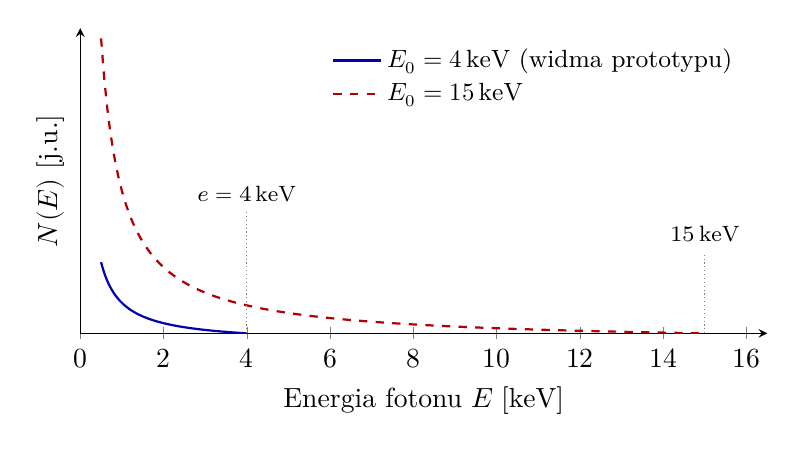
\begin{tikzpicture}
    \begin{axis}[
        width=0.85\linewidth, height=0.45\linewidth,
        xmin=0, xmax=16.5, ymin=0, ymax=30,
        xlabel={Energia fotonu $E$ [\si{\kilo\electronvolt}]},
        ylabel={$N(E)$ [j.u.]},
        ytick=\empty, axis lines=left,
        legend style={draw=none, font=\small}, legend cell align=left, legend pos=north east]
      \addplot[thick, blue!70!black, domain=0.5:4, samples=120]
        {(4-x)/x};
      \addlegendentry{$E_0=\SI{4}{\kilo\electronvolt}$ (widma prototypu)}
      \addplot[thick, red!70!black, dashed, domain=0.5:15, samples=200]
        {(15-x)/x};
      \addlegendentry{$E_0=\SI{15}{\kilo\electronvolt}$}
      \draw[gray, densely dotted] (axis cs:4,0) -- (axis cs:4,12)
        node[above, font=\footnotesize, black] {$e\UT=\SI{4}{\kilo\electronvolt}$};
      \draw[gray, densely dotted] (axis cs:15,0) -- (axis cs:15,8)
        node[above, font=\footnotesize, black] {\SI{15}{\kilo\electronvolt}};
    \end{axis}
  \end{tikzpicture}
  \caption{Widmo promieniowania hamowania według wzoru Kramersa dla dwóch
    energii elektronów; widmo kończy się na granicy Duane'a--Hunta
    $E_\mathrm{max}=eU$. Na widmo ciągłe nakładają się linie
    charakterystyczne, a~przy małych energiach jest ono osłabiane przez
    absorpcję w~próbce i~oknie detektora \opracowanieWlasne}
  \label{fig:kramers}
\end{figure}

\subsection{Jonizacja powłok wewnętrznych}
\label{subsec:jonizacja}

Elektron wiązki może wybić elektron z~wewnętrznej powłoki atomu (K, L,
M), jeśli jego energia jest większa od energii wiązania tej powłoki,
nazywanej energią krytyczną $E_\mathrm{c}$ (odpowiada ona krawędzi
absorpcji). Na przykład dla powłoki K krzemu
$E_\mathrm{c}=\SI{1.84}{\kilo\electronvolt}$, a~dla żelaza
\SI{7.11}{\kilo\electronvolt}. Stosunek energii elektronów do energii
krytycznej nazywa się współczynnikiem nadnapięcia
\begin{equation}
  U_0 = \frac{E_0}{E_\mathrm{c}}.
\end{equation}
Natężenie linii charakterystycznej rośnie w~przybliżeniu jak
$(U_0-1)^{n}$, gdzie $n\approx1{,}5$--$1{,}7$. W~praktyce do skutecznego
wzbudzenia linii stosuje się $U_0\approx2$--3. Przy napięciu
przyspieszającym \SI{15}{\kilo\volt} dobrze wzbudzane są linie K
pierwiastków do żelaza włącznie, co obejmuje główne pierwiastki
skałotwórcze (O, Mg, Al, Si, Ca, Fe). Przy energii
\SI{4}{\kilo\electronvolt}, stosowanej przy rejestracji widm prototypu,
warunek $U_0\geq2$ spełniają linie K pierwiastków o~energii krytycznej do
ok. \SI{2}{\kilo\electronvolt}: O, Na, Mg, Al i~Si. Linie K fosforu
i~siarki są wzbudzane słabiej ($U_0\approx1{,}6$--1{,}9), linia K potasu
tylko śladowo, a~linii K wapnia ($E_\mathrm{c}=\SI{4.04}{\kilo\electronvolt}$)
i~linii K żelaza ($E_\mathrm{c}=\SI{7.11}{\kilo\electronvolt}$) nie da się wzbudzić.
Żelazo i~inne metale przejściowe można wtedy rozpoznać tylko po liniach L
(np. Fe L$\alpha$ \SI{0.705}{\kilo\electronvolt}). Pomiary emisji przy
$U_\mathrm{T}=\SI{2}{\kilo\volt}$ służyły do badania źródła elektronów,
a~nie do analizy widma.

\subsection{Relaksacja atomu i~emisja fotonu promieniowania X}

Po jonizacji powłoki wewnętrznej atom znajduje się w~stanie wzbudzonym.
Lukę zapełnia elektron z~wyższej powłoki, a~nadmiar energii, równy
różnicy energii wiązania obu powłok, zostaje wypromieniowany jako foton
promieniowania X. Energie powłok są inne dla każdego pierwiastka, dlatego
energia fotonu jest cechą charakterystyczną pierwiastka i~na niej opiera
się identyfikacja składu w~spektroskopii EDS. Przykładowo przejście
elektronu z~powłoki L na powłokę K w~atomie glinu daje foton Al~\Ka{}
o~energii \SI{1.486}{\kilo\electronvolt}.

Nie każda relaksacja kończy się emisją fotonu. W~konkurencyjnym efekcie
Augera nadmiar energii przejmuje inny elektron atomu, który opuszcza atom,
i~foton nie powstaje. Udział relaksacji z~emisją fotonu opisuje wydajność
fluorescencji $\omega$, rosnąca z~liczbą atomową: dla powłoki K krzemu
wynosi ok.~\num{0.05}, a~dla żelaza ok.~\num{0.35}. Lekkie pierwiastki
emitują więc mniej fotonów na jedną jonizację i~dają w~widmie słabsze
linie~\cite{goldstein2018sem,beckhoff2006xrf}.

\subsection{Nazewnictwo linii i~prawo Moseleya}

Linie oznacza się literą powłoki, na której powstała luka, oraz
indeksem określającym, skąd pochodzi elektron zapełniający:
K$\alpha$ (przejście L$\to$K), K$\beta$ (M$\to$K), L$\alpha$ (M$\to$L)
itd. (notacja Siegbahna; w~notacji IUPAC np. K$\alpha_1$ = K--L$_3$).
Energia linii zależy od liczby atomowej zgodnie z~prawem Moseleya.
Dla linii K$\alpha$ w~przybliżeniu
\begin{equation}
  E_{\mathrm{K}\alpha} \approx \SI{10.2}{\electronvolt}\,(Z-1)^2,
\end{equation}
co np. dla żelaza ($Z=26$) daje ok. \SI{6.4}{\kilo\electronvolt},
zgodnie z~wartością tablicową. Jednoznaczna zależność energii linii od
$Z$ jest podstawą identyfikacji pierwiastków w~widmie.
Przykładowe energie linii K$\alpha$: O~\SI{0.525}{\kilo\electronvolt},
Mg \SI{1.254}{\kilo\electronvolt}, Al \SI{1.487}{\kilo\electronvolt},
Si \SI{1.740}{\kilo\electronvolt}, Ca \SI{3.69}{\kilo\electronvolt},
Fe \SI{6.40}{\kilo\electronvolt}.

\subsection{EDS a~XRF}

Obie metody rejestrują to samo promieniowanie charakterystyczne, ale
różnią się sposobem wzbudzenia:
\begin{itemize}
  \item w~\textbf{EDS} (w~mikroskopie elektronowym) próbkę wzbudza wiązka
        elektronów. Wiązkę łatwo zogniskować do małej plamki
        i~wydajnie wzbudza ona pierwiastki lekkie, ale towarzyszy jej
        silne tło promieniowania hamowania, a~próbka nieprzewodząca może
        się ładować;
  \item w~\textbf{XRF} próbkę wzbudzają fotony promieniowania X (z~lampy
        rentgenowskiej lub izotopu). Tło jest znacznie mniejsze, bo nie
        powstaje promieniowanie hamowania w~próbce, ale wzbudzenie
        pierwiastków lekkich jest słabsze, a~ogniskowanie promieniowania
        X wymaga specjalnej optyki~\cite{beckhoff2006xrf}.
\end{itemize}
Miniaturowe źródło RTG MEMS rozwijane na Politechnice Wrocławskiej
zastosowano dotychczas do spektrometrii XRF~\cite{urbanski2026xrf}.
W~tej pracy wiązka elektronów pada bezpośrednio na próbkę, czyli
przyrząd działa jak analizator EDS.

\subsection{Target transmisyjny i~odbiciowy}
\label{subsec:target}

W~źródle rentgenowskim wiązka elektronów pada na target. W~targecie
odbiciowym promieniowanie wyprowadza się od strony padania wiązki, pod
kątem do jej osi. W~targecie transmisyjnym warstwa metalu (np. W, Mo)
jest naniesiona na cienką membranę, a~promieniowanie wychodzi na wylot,
wzdłuż osi wiązki. Grubość warstwy dobiera się tak, aby była porównywalna
z~zasięgiem elektronów: zbyt cienka nie wykorzysta energii wiązki, zbyt
gruba pochłonie wytworzone promieniowanie. Konstrukcja transmisyjna
pozwala zbudować źródło osiowe i~zwarte, dlatego zastosowano ją w~źródle
MEMS~\cite{urbanski2023target,urbanski2024monochromatic}. W~analizatorze
EDS rolę targetu pełni badana próbka.

% =====================================================================
\section{Pomiar widma metodą EDS}
\label{sec:spektrometria}

\subsection{Stanowisko pomiarowe}

Stanowisko składa się z~komory próżniowej z~układem pomp, badanej
struktury (emiter, bramka, target lub próbka), dwóch zasilaczy
wysokiego napięcia (obwód bramki i~obwód targetu), rezystorów
ograniczających \SI{100}{\kilo\ohm} z~woltomierzami do pomiaru prądów
oraz spektrometru rentgenowskiego ustawionego tak, aby widział
oświetlany obszar próbki. Ciśnienie w~komorze podczas pomiarów wynosiło
ok. \SI{1e-5}{\hecto\pascal}. Charakterystyki emisji mierzono przy
$U_\mathrm{T}=\SI{2000}{\volt}$, a~widma przy
$U_\mathrm{T}=\SI{4000}{\volt}$ i~$U_\mathrm{B}=\SI{1000}{\volt}$.
Schemat elektryczny przedstawiono na rys.~\ref{fig:uklad-pomiarowy}.

\subsection{Charakterystyka prądowo-napięciowa emitera}

Podstawowym pomiarem źródła elektronów jest zależność prądu emisji od
napięcia bramki $I(U_\mathrm{B})$ przy stałym $U_\mathrm{T}$.
Z~charakterystyki odczytuje się napięcie progowe i~maksymalny stabilny
prąd. Wykres F--N służy do potwierdzenia mechanizmu emisji. Pomiary
porównawcze z~magnesem i~bez magnesu oraz przed i~po odgazowaniu
pokazują wpływ ogniskowania i~stanu powierzchni emitera.

\subsection{Półprzewodnikowy detektor promieniowania X}

Foton promieniowania X pochłonięty w~krysztale półprzewodnika wytwarza
pary elektron--dziura. Średnia energia na wytworzenie jednej pary
w~krzemie wynosi $\varepsilon\approx\SI{3.6}{\electronvolt}$, więc foton
o~energii \SI{6}{\kilo\electronvolt} wytwarza ok. 1600 par. Pole
elektryczne w~detektorze rozdziela nośniki, zanim zdążą zrekombinować,
i~zbiera je na elektrodach. Zebrany ładunek jest proporcjonalny do
energii fotonu~\cite{urbanski2023detection}.

Stosowane typy detektorów:
\begin{itemize}
  \item \textbf{Si(Li)} -- krzem kompensowany litem, wymaga chłodzenia
        ciekłym azotem,
  \item \textbf{SDD} (krzemowy detektor dryfowy) -- elektrony dryfują do
        małej anody o~niskiej pojemności, co obniża szumy i~pozwala na
        duże szybkości zliczeń. Chłodzony ogniwem Peltiera, obecnie
        najczęściej stosowany,
  \item \textbf{CdTe} -- wyższa liczba atomowa, lepsza wydajność dla
        energii powyżej ok. \SI{20}{\kilo\electronvolt}, gorsza
        rozdzielczość.
\end{itemize}
Typ detektora w~spektrometrze użytym do pomiarów nie był znany, dlatego
w~pracy opisano zasadę działania detektorów półprzewodnikowych ogólnie.

\subsection{Tor akwizycji}

Ładunek z~detektora jest zamieniany na impuls napięciowy przez
przedwzmacniacz ładunkowy. Układ kształtujący (obecnie cyfrowy procesor
impulsów) filtruje sygnał i~mierzy amplitudę każdego impulsu.
Analizator wielokanałowy (MCA) przypisuje impuls do kanału odpowiadającego
jego amplitudzie i~zlicza impulsy w~kanałach. Wynikiem jest histogram
liczby zliczeń w~funkcji energii, czyli widmo.

\subsection{Analiza widma}

Analiza jakościowa polega na przypisaniu pikom pierwiastków na
podstawie energii linii. Należy uwzględnić zjawiska, które dają piki
pozorne lub zniekształcenia:
\begin{itemize}
  \item \textbf{tło promieniowania hamowania}, które trzeba odjąć przed
        wyznaczeniem pola powierzchni pików,
  \item \textbf{piki ucieczki} -- foton padający wzbudza w~detektorze
        krzemowym promieniowanie Si K$\alpha$, które ucieka z~kryształu.
        Rejestrowana jest wtedy energia mniejsza o~\SI{1.74}{\kilo\electronvolt},
  \item \textbf{piki sumacyjne} -- dwa fotony zarejestrowane niemal
        jednocześnie dają impuls o~sumie ich energii,
  \item \textbf{nakładanie się linii} różnych pierwiastków o~zbliżonych
        energiach (np. S K$\alpha$ \SI{2.31}{\kilo\electronvolt}
        i~Mo L$\alpha$ \SI{2.29}{\kilo\electronvolt}),
  \item \textbf{linie pochodzące z~elementów konstrukcji} (bramka,
        uchwyt, ścianki komory), w~które trafiają elektrony rozproszone.
\end{itemize}

\subsection{EDS a~WDS}

Oprócz spektrometrii z~dyspersją energii (EDS) stosuje się spektrometrię
z~dyspersją długości fali (WDS). Energia fotonu i~długość fali są
związane zależnością
\begin{equation}
  E\,[\si{\kilo\electronvolt}] = \frac{hc}{\lambda} \approx \frac{1{,}2398}{\lambda\,[\si{\nano\metre}]}.
\end{equation}
W~WDS promieniowanie odbija się od kryształu analizatora i~do detektora
dociera tylko długość fali spełniająca warunek Bragga
\begin{equation}
  n\lambda = 2d\sin\theta,
\end{equation}
gdzie $d$ jest odległością płaszczyzn sieciowych, a~$\theta$ kątem
padania. Widmo mierzy się, zmieniając kąt. WDS ma rozdzielczość rzędu
\SI{10}{\electronvolt}, ale wymaga ruchomego goniometru, rejestruje
naraz jedną linię i~jest duży. EDS rejestruje całe widmo jednocześnie
w~małym detektorze bez części ruchomych, dlatego tylko ta metoda nadaje
się do miniaturowego przyrządu kosmicznego~\cite{goldstein2018sem}.

\subsection{Analiza ilościowa}

Skład ilościowy wyznacza się z~natężeń linii, porównując je z~natężeniami
zmierzonymi dla wzorców o~znanym składzie. Wymaga to poprawek na liczbę
atomową, absorpcję i~fluorescencję wtórną w~próbce (poprawki ZAF) oraz
płaskiej, wypolerowanej powierzchni próbki i~stabilnego prądu wiązki.
W~tej pracy prąd wiązki i~geometria pomiaru nie były na tyle stabilne
i~znane, aby prowadzić analizę ilościową, dlatego ograniczono się do
analizy jakościowej.

\subsection{Niepewność pomiaru}

Zliczenia fotonów podlegają rozkładowi Poissona, więc niepewność liczby
zliczeń $N$ w~piku wynosi $\sqrt{N}$, a~niepewność względna $1/\sqrt{N}$.
Do uzyskania niepewności względnej \SI{1}{\percent} potrzeba ok.
\num{10000} zliczeń w~piku. Niepewność pomiaru prądu wynika z~klasy
woltomierza i~tolerancji rezystora (\SI{100}{\kilo\ohm}), a~niepewność
napięć z~dokładności zasilaczy.

% =====================================================================
\section{Zagadnienia uzupełniające}
\label{sec:uzupelnienia}

\subsection{Próżnia}

Elektrony muszą przebyć drogę od emitera do próbki bez zderzeń
z~cząsteczkami gazu. Średnia droga swobodna cząsteczki powietrza
w~temperaturze pokojowej wynosi w~przybliżeniu
$\lambda\,[\si{\milli\metre}] \approx 6{,}6/p\,[\si{\pascal}]$,
a~dla elektronu jest ok. 5--6 razy większa. Przy ciśnieniu
\SI{1e-3}{\pascal} (\SI{1e-5}{\hecto\pascal}) droga swobodna elektronu
wynosi kilkadziesiąt metrów, czyli wielokrotnie więcej niż wymiary
struktury. Niskie ciśnienie jest potrzebne także ze względu na trwałość
emitera (bombardowanie jonowe, adsorpcja gazów) i~ryzyko wyładowań między
elektrodami.

W~tej pracy próżnię zapewniała komora próżniowa.
W~docelowej strukturze hermetycznej (p.~\ref{subsec:bonding}) próżnię
podtrzymywałaby zintegrowana mikropompa jonowo-sorpcyjna. Wiązka
elektronów wywołuje desorpcję gazów ze ścianek (desorpcja stymulowana
elektronami), więc sama hermetyzacja nie wystarcza do utrzymania próżni
\cite{grzebyk2014micropump,grzebyk2017pumps,urbanski2026phd}.

\subsection{Warunki pracy w~misji kosmicznej}
\label{subsec:warunki}

Na powierzchni Księżyca i~planetoid panuje naturalna próżnia (na
Księżycu rzędu \SI{1e-10}{\pascal}), wystarczająca do propagacji wiązki
elektronów bez osobnej komory. Na Marsie ciśnienie atmosfery CO$_2$
wynosi ok. \SI{600}{\pascal}, więc wiązka elektronów musiałaby przejść
przez cienkie okno lub krótki odcinek gazu. Rozwiązania tego typu
rozważano dla miniaturowych mikroskopów ze zmiennym ciśnieniem
\cite{gaskin2012mvpsem,thaisen2010minisem}.
Przyrząd musi ponadto znosić promieniowanie kosmiczne, duże zmiany
temperatury i~przeciążenia przy starcie, a~jego masa i~pobór mocy są
ograniczone budżetem misji.

\subsection{Porównanie z~przyrządami stosowanymi w~misjach}

Analizę składu pierwiastkowego in situ prowadzą obecnie:
\begin{itemize}
  \item \textbf{APXS} (łaziki MER i~Curiosity) -- wzbudzanie
        izotopem $^{244}$Cm (cząstki alfa i~promieniowanie X), detektor
        SDD; pomiar trwa od kilkunastu minut do kilku godzin
        \cite{rieder2003apxs,campbell2012apxs,gellert2015apxs},
  \item \textbf{PIXL} (Perseverance) -- mikro-XRF z~lampą rentgenowską
        i~optyką polikapilarną, wiązka o~średnicy ok.
        \SI{120}{\micro\metre}, mapowanie składu~\cite{allwood2020pixl},
  \item \textbf{CheMin} (Curiosity) -- dyfrakcja i~fluorescencja
        rentgenowska próbek pobranych przez łazik~\cite{blake2012chemin}.
\end{itemize}
Żaden z~nich nie wzbudza próbki bezpośrednio wiązką elektronów.
Analizator EDS z~katodą polową w~technologii MEMS mógłby uzupełnić te
przyrządy jako lekki czujnik o~małym poborze mocy, przeznaczony na
powierzchnię ciał bez atmosfery.

\subsection{Elektronika zasilania i~sterowania}

Źródło wymaga dwóch napięć: ekstrakcyjnego (rzędu \SI{1}{\kilo\volt})
i~przyspieszającego (rzędu \SIrange{10}{20}{\kilo\volt}). W~przyrządach
przenośnych i~kosmicznych wysokie napięcie uzyskuje się z~przetwornicy
z~transformatorem podwyższającym i~powielaczem napięcia
Cockcrofta--Waltona, co pozwala zmieścić zasilacz w~małej objętości.
Ponieważ prąd emisji polowej zmienia się wykładniczo z~napięciem i~jest
wrażliwy na stan powierzchni emitera, w~docelowym przyrządzie potrzebna
jest pętla sprzężenia zwrotnego, która mierzy prąd wiązki i~koryguje
napięcie ekstrakcyjne. Pozwala to utrzymać stałą liczbę zliczeń
w~widmie i~chroni emiter przed przeciążeniem. Układ sterujący
odpowiadałby też za rejestrację widma i~jego wstępne przetwarzanie
(identyfikację linii) przed wysłaniem danych na Ziemię.

\subsection{Bezpieczeństwo pracy}

Podczas pomiarów występują dwa zagrożenia: wysokie napięcie i~promieniowanie
X. Zasilacze wysokiego napięcia muszą mieć ograniczenie prądu, a~obwody
-- rezystory ograniczające. Przy napięciach przyspieszających do ok.
\SI{20}{\kilo\volt} promieniowanie X jest miękkie i~skutecznie pochłaniane
przez metalowe ścianki komory. Okna (np. z~berylu lub szkła) są miejscami,
przez które promieniowanie może wydostawać się na zewnątrz, dlatego przy
pracy źródła należy zachować odległość i~ograniczyć czas przebywania
w~pobliżu okien.

        % 9. wprowadzenie teoretyczne
% Rozdział 3 — Projekt i wykonanie prototypu (budżet: 6,5 str.)
% Źródło: projekt-prototypu/projekt.tex (ma własne \chapter i \label{ch:projekt}).
% Plan akapitów i brakujące dane (T1–T20): wspolne/rozdzial3_plan.md
% =====================================================================
%  Rozdział 3 — Projekt i wykonanie prototypu (budżet: 6,5 str., ok. 1500 słów)
%  Plan akapitów: wspolne/rozdzial3_plan.md (oznaczenia T1–T20 = brakujące dane)
%  Wersja robocza 09.11.2026: napisane 3.1 i 3.2 (budowa struktury, szkło 1 mm),
%  pozostałe podrozdziały jako nagłówki z \TODO.
% =====================================================================
\chapter{Projekt i~wykonanie prototypu}
\label{ch:projekt}

W~rozdziale opisano projekt struktury krzemowo-szklanej źródła elektronów
oraz kolejne etapy jej wytworzenia, aż do zmontowanego prototypu. Zasady
zastosowanych procesów technologicznych omówiono w~\pref{sec:technologia},
a~stanowisko pomiarowe w~\rozdzref{ch:stanowisko}.

% ---------------------------------------------------------------------
\section{Założenia projektowe i~koncepcja struktury}
\label{sec:koncepcja}

Prototyp miał spełniać następujące wymagania:
\begin{itemize}[nosep]
  \item wytworzenie wiązki elektronów przez emisję polową z~nanorurek
        węglowych przy napięciu ekstrakcyjnym $\UB$ rzędu \SI{1}{\kilo\volt},
  \item przyspieszenie elektronów do energii wystarczającej do wzbudzenia
        linii charakterystycznych pierwiastków lekkich (w~badaniach
        $\UT$ do \SI{4}{\kilo\volt}, docelowo \SIrange{10}{18}{\kilo\volt}),
  \item izolacja elektryczna elektrod przy tych napięciach,
  \item wykonanie wyłącznie procesami MEMS: fotolitografią, trawieniem
        krzemu i~bondingiem anodowym krzem--szkło,
  \item możliwość późniejszej hermetyzacji struktury.
\end{itemize}

Strukturę zaprojektowano jako stos płaskich elementów krzemowych
rozdzielonych szkłem borokrzemowym (\rysref{fig:przekroj-struktury}).
Licząc od dołu, składa się ona z~emitera (E) z~ostrzem uformowanym
z~nanorurek węglowych, szkła dystansowego o~grubości \SI{1}{\milli\metre},
bramki (elektrody ekstrakcyjnej, B), drugiego szkła dystansowego oraz
targetu (T). Każda elektroda krzemowa jest osobnym elementem
z~własnym kontaktem elektrycznym, a~szkło oddziela je galwanicznie
i~ustala odległości między nimi. Wiązkę ogniskuje magnes trwały NdFeB
umieszczony przy emiterze
\TODO{T1: położenie magnesu i~ewentualne dodatkowe elementy wg szkicu}.

\begin{figure}[htbp]
  \centering
  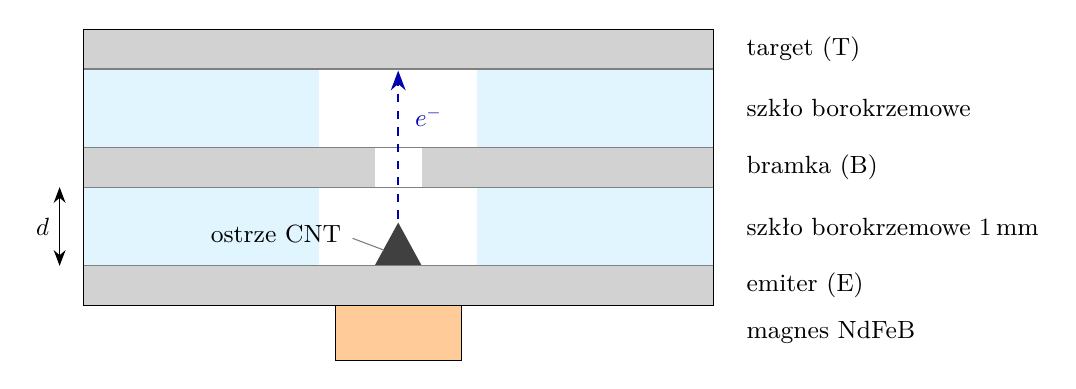
\begin{tikzpicture}[x=1cm, y=1cm, font=\small]
    % kolory
    \colorlet{si}{gray!35}
    \colorlet{gl}{cyan!12}
    % target
    \fill[si] (0,4.4) rectangle (8,4.9);
    % szkło 2 z otworem
    \fill[gl] (0,3.4) rectangle (3,4.4);
    \fill[gl] (5,3.4) rectangle (8,4.4);
    % bramka z aperturą
    \fill[si] (0,2.9) rectangle (3.7,3.4);
    \fill[si] (4.3,2.9) rectangle (8,3.4);
    % szkło 1 z otworem
    \fill[gl] (0,1.9) rectangle (3,2.9);
    \fill[gl] (5,1.9) rectangle (8,2.9);
    % emiter
    \fill[si] (0,1.4) rectangle (8,1.9);
    % wieża (ostrze) CNT
    \fill[black!75] (3.7,1.9) -- (4,2.45) -- (4.3,1.9) -- cycle;
    % magnes (poglądowo, położenie do potwierdzenia)
    \fill[orange!40] (3.2,0.7) rectangle (4.8,1.4);
    % obrysy
    \foreach \y in {1.4,1.9,2.9,3.4,4.4,4.9} {\draw[gray] (0,\y) -- (8,\y);}
    \draw (0,1.4) rectangle (8,4.9);
    \draw (3.2,0.7) rectangle (4.8,1.4);
    % wiązka
    \draw[-{Stealth[length=2.5mm]}, blue!70!black, thick, dashed]
      (4,2.5) -- (4,4.38);
    % opisy
    \foreach \y/\t in {4.65/target (T),
                       3.9/szkło borokrzemowe,
                       3.15/bramka (B),
                       2.4/szkło borokrzemowe \SI{1}{\milli\metre},
                       1.65/emiter (E),
                       1.05/magnes NdFeB}
      {\node[anchor=west] at (8.3,\y) {\t};}
    \node[anchor=east] at (3.4,2.3) {ostrze CNT};
    \draw[gray] (3.42,2.25) -- (3.82,2.1);    \node[anchor=west, blue!70!black] at (4.1,3.75) {$e^-$};
    % wymiar
    \draw[{Stealth[length=2mm]}-{Stealth[length=2mm]}] (-0.3,1.9) -- (-0.3,2.9)
      node[midway, left] {$d$};
  \end{tikzpicture}
  \caption{Przekrój struktury prototypu (schemat poglądowy, bez zachowania
    skali): E -- emiter z~ostrzem CNT, B -- bramka (elektroda ekstrakcyjna),
    T -- target; $d$ -- odległość emiter--bramka \opracowanieWlasne}
  \label{fig:przekroj-struktury}
\end{figure}
% TODO(rys.): podmienić na wersję zgodną ze szkicem kris (T1); sprawdzić
% grubość drugiego szkła, kształt emitera, wymiary otworów i położenie magnesu.

W~porównaniu ze źródłem promieniowania rentgenowskiego opisanym
w~\cite{urbanski2026phd} konstrukcja jest uproszczona: nie ma
elektrody ogniskującej ani zintegrowanej mikropompy, a~wiązka pada
bezpośrednio na target, który pełni rolę nośnika badanej próbki
(lub warstwy luminoforu), a~nie targetu transmisyjnego.
Sposób zasilania elektrod opisano w~\rozdzref{ch:stanowisko}.
\TODO{T2: które elementy przejęto z~projektu źródła RTG, a~które zaprojektowano od nowa}

% ---------------------------------------------------------------------
\section{Dobór materiałów i~grubości elementów}
\label{sec:materialy}

Elektrody wykonano z~płytek krzemu monokrystalicznego o~orientacji
(100), ponieważ kształt emitera i~otworów uzyskuje się trawieniem
anizotropowym (\pref{subsec:koh}), a~krzem jest jednocześnie materiałem
konstrukcyjnym i~przewodzącym.
\TODO{T4: grubość, typ i~rezystywność płytek Si}

Jako dystansownik między emiterem a~bramką zastosowano szkło
borokrzemowe o~grubości \SI{1}{\milli\metre}. Grubość szkła wyznacza
bezpośrednio odległość emiter--bramka $d$, a~więc natężenie pola
elektrycznego przy emiterze. Przy $d \approx \SI{1}{\milli\metre}$
i~$\UB = \SI{1}{\kilo\volt}$ średnie natężenie pola wynosi ok.
\SI{1}{\volt\per\micro\metre}; lokalne pole na wierzchołkach nanorurek
jest wielokrotnie większe dzięki współczynnikowi wzmocnienia pola
(\pref{sec:emisja}). Ostrze CNT o~wysokości $h$ skraca odległość
wierzchołka od bramki do $d - h$, co dodatkowo zwiększa pole przy
wierzchołku.
\TODO{T7: wysokość ostrza CNT $h$ i~średnica apertury bramki}

Drugim zadaniem szkła jest izolacja elektrod. W~próżni ograniczeniem
jest przede wszystkim przeskok wzdłuż powierzchni szkła między krawędziami
sąsiednich elektrod, dlatego grubość dystansownika wyznacza też drogę
upływu. Między bramką a~targetem występuje różnica potencjałów
$\UT - \UB$, a~między emiterem a~bramką $\UB$. Przy napięciach
stosowanych w~badaniach (do \SI{4}{\kilo\volt}) szkło o~grubości
\SI{1}{\milli\metre} zapewniało wystarczającą izolację. Przy docelowych
napięciach \SIrange{10}{18}{\kilo\volt} potrzebne są dodatkowe
zabezpieczenia, np. zalanie krawędzi struktury żywicą epoksydową, jak
w~\cite{urbanski2026phd}.
\TODO{T5: typ szkła (Borofloat~33?), grubość drugiego szkła, powód wyboru 1~mm}

Szkło borokrzemowe ma współczynnik rozszerzalności cieplnej zbliżony do
krzemu i~zawiera jony sodu, dzięki czemu można je łączyć z~krzemem
bondingiem anodowym (\pref{subsec:bonding}). Duża odległość między
emiterem a~targetem sprzyja jednak rozbieganiu się wiązki, co uzasadnia
zastosowanie magnesu ogniskującego (\pref{sec:wiazka}).
Wymiary wszystkich elementów zestawiono w~\tabref{tab:elementy-struktury}.

\begin{table}[htbp]
  \centering
  \caption{Elementy struktury prototypu (od dołu)}
  \label{tab:elementy-struktury}
  \begin{tabular}{@{}llll@{}}
    \toprule
    Element & Materiał & Grubość & Funkcja \\
    \midrule
    emiter (E)        & Si (100) + ostrze CNT & \TODO{T4}          & źródło elektronów \\
    dystansownik      & szkło borokrzemowe   & \SI{1}{\milli\metre} & izolacja, odległość $d$ \\
    bramka (B)        & Si (100)             & \TODO{T4}           & elektroda ekstrakcyjna \\
    dystansownik      & szkło borokrzemowe   & \TODO{T5}           & izolacja B--T \\
    target (T)        & \TODO{T8}            & \TODO{T8}           & nośnik próbki / luminoforu \\
    magnes ogniskujący & NdFeB               & --                  & ogniskowanie wiązki \\
    \bottomrule
  \end{tabular}
\end{table}

% ---------------------------------------------------------------------
\section{Projekt emitera, bramki i~targetu}
\label{sec:projekt-elektrod}
\TODO{T6--T8: wymiary emitera, apertura bramki, target; magnes jakościowo (plan p.~3.3)}

\section{Projekt masek fotolitograficznych}
\label{sec:maski}
\TODO{T9--T10: liczba i~przeznaczenie masek, reguły projektowe, rozkład na płytce (plan p.~3.4)}

\section{Wytwarzanie elementów krzemowych}
\label{sec:wytwarzanie-si}
\TODO{T11--T14: warstwa maskująca, fotolitografia, trawienie KOH, kontrola wymiarów (plan p.~3.5)}

\section{Wykonanie elementów szklanych}
\label{sec:szklo}

Dystansowniki wykonano z~płytki szkła borokrzemowego o~grubości
\SI{1}{\milli\metre}. Najpierw wytrawiono w~niej otwory o~średnicy
\SI{0.6}{\milli\metre}, przez które przechodzi wiązka elektronów,
a~następnie płytkę pocięto piłą na pojedyncze elementy. Taka kolejność
pozwala obrabiać całą płytkę naraz i~zachować jednakowe położenie
otworów we wszystkich dystansownikach. Przed bondingiem elementy
oczyszczono, ponieważ zanieczyszczenia i~nierówności powierzchni
uniemożliwiają szczelne połączenie (\pref{subsec:bonding}).
\TODO{T15: roztwór i~maska do trawienia otworów w~szkle, sposób czyszczenia}

\section{Formowanie emitera CNT}
\label{sec:nanoszenie-cnt}

Emiter ma postać ostrza (wieży) z~nanorurek węglowych na płaskim
elemencie krzemowym. Zawiesinę nanorurek nakraplano pipetą na element
pomocniczy, który przykładano do emitera nagrzanego na płycie grzejnej
do \SI{240}{\celsius}. Element pomocniczy odciągano następnie szybkim
ruchem od powierzchni emitera. Zawiesina rozciągała się między oboma
elementami i~zasychała w~kontakcie z~gorącym podłożem, tworząc wieżę
nanorurek wydłużoną w~kierunku przyszłej bramki. Kształt ostrza
zwiększa lokalne natężenie pola na jego wierzchołku i~skraca odległość
od bramki (\pref{sec:materialy}).
\TODO{T16: skład zawiesiny (rodzaj CNT, rozpuszczalnik, PVP?), materiał elementu pomocniczego, wysokość i~średnica uzyskanej wieży}
\TODO{T17: czy emiter formowano przed bondingiem, czy po nim}

\section{Bonding anodowy i~montaż prototypu}
\label{sec:bonding-montaz}

Elementy połączono bondingiem anodowym w~atmosferze. Stół grzejny
nagrzewano do \SI{450}{\celsius}, czyli do górnej granicy typowego
zakresu temperatur procesu (\pref{subsec:bonding}). Stół był
jednocześnie elektrodą uziemiającą, a~kolejne warstwy stosu znajdowały
się coraz dalej od niego, więc ich temperatura była niższa niż
temperatura stołu. Wysoka temperatura stołu zapewniała, że także
najwyżej położone połączenia osiągały temperaturę wystarczającą do
przewodnictwa jonowego szkła. Między elementy wprowadzono dodatkowo
przekładkę, która zmniejszała dystans między łączonymi elementami.
\TODO{T18: kolejność łączenia warstw, sposób justowania otworów względem ostrza; czym była przekładka i~gdzie leżała}
\TODO{T19: napięcie i~czas bondingu, czy wszystkie połączenia były trwałe}

\TODO{T20: montaż -- położenie magnesu, kontakty elektryczne do E, B, T, luminofor i~próbka na targecie, wymiary i~masa prototypu}

Wszystkie połączenia wykonano w~atmosferze, dlatego wnętrze struktury
nie jest zamknięte w~próżni, a~prototyp jest niehermetyczny. Badania
prowadzono w~komorze próżniowej przy ciśnieniu ok.
\SI{1e-5}{\hecto\pascal} (\rozdzref{ch:stanowisko}). Rozwiązaniem
docelowym jest wykonanie ostatniego połączenia bondingiem anodowym
w~próżni i~podtrzymywanie próżni mikropompą; trudności tego procesu
omówiono w~\pref{subsec:bonding}.

         % 10. prace własne
% Rozdział 4 — Stanowisko pomiarowe i metodyka (budżet: 3,5 str.)
% Źródła: uklad-pomiarowy/uklad_pomiarowy_body.tex (schemat circuitikz,
% samodzielny dokument — wstawiany makrem \inputBezPreambuly, bez zmian w pliku).
% Podpis jak w uklad-pomiarowy/rysunek_w_pracy.tex, ze ścieżką i nazwą
% dopasowaną do pracy (słownik N6, N9). Docelowo wątek rozdziału
% przenosi ten blok do własnego pliku.
\chapter{Stanowisko pomiarowe i~metodyka}
\label{ch:stanowisko}
\TODO{opis komory próżniowej, obwodu E--B--T, spektrometru, metody analizy zdjęć}

\begin{figure}[htbp]
  \centering
  \resizebox{\textwidth}{!}{\inputBezPreambuly{../uklad-pomiarowy/uklad_pomiarowy_body}}
  \caption{Schemat układu do pomiaru emisji polowej w~prototypie analizatora EDS:
    E -- emiter, B -- bramka (elektroda ekstrakcyjna), T -- target;
    $\UT$ -- zasilacz obwodu targetu, $\UB$ -- zasilacz bramki;
    $\RT$, $\RB$ -- rezystory ograniczające, V -- woltomierze
    \opracowanieWlasne}
  \label{fig:uklad-pomiarowy}
\end{figure}

% Rozdział 5 — Badania eksperymentalne (budżet: 13 str.)
% 5.1 Źródło: emisja-magnes-pomiary/emisja_tresc.tex (zaczyna się od \section).
% Fragment używa \figdir i \datadir — ustawiane tutaj względem wspolne/.
\chapter{Badania eksperymentalne}
\label{ch:badania}

\renewcommand{\figdir}{../emisja-magnes-pomiary/figures}
\renewcommand{\datadir}{../emisja-magnes-pomiary/dane}
% =====================================================================
%  Emisja polowa: sesja z magnesem vs. sesje bez magnesu
%  Fragment do wstawienia w rozdział 5 (\input{...}).
%  Wymaga: graphicx, subcaption, pgfplots (compat>=1.17), booktabs, siunitx
%  Ścieżki: figures/ (zdjęcia), dane/ (CSV z pomiarów i analizy obrazu)
% =====================================================================
\providecommand{\sesjaM}{z~magnesem}
\providecommand{\sesjaB}{bez magnesu}
\providecommand{\figdir}{figures}
\providecommand{\datadir}{dane}
\pgfplotsset{/pgf/number format/use comma, /pgf/number format/1000 sep={}}
\providecommand{\TODO}[1]{\textcolor{red}{[TODO: #1]}}

\section{Wpływ magnesu ogniskującego na emisję polową}
\label{sec:emisja-magnes}

\subsection{Przebieg pomiarów}

Porównano dwie sesje pomiarowe, w~których przy stałym napięciu targetu
zwiększano napięcie $U$ co \SI{100}{V} i~rejestrowano prąd emisji
$I_e$ oraz zdjęcie ekranu luminescencyjnego:
\begin{itemize}
  \item \textbf{Sesja B} (\sesjaB) -- napięcie targetu \SI{2000}{V},
        $U=\SIrange{500}{1500}{V}$, prąd w~zakresie
        \SIrange{2}{22}{\micro A};
        zdjęcia dla $U=\SIrange{700}{1100}{V}$ (arkusz \emph{Book1},
        seria~1). Przed tą sesją źródło zostało odgazowane przez
        wygrzanie w~temperaturze ok. \SI{200}{\celsius}.
  \item \textbf{Sesja M} (\sesjaM) -- napięcie targetu \SI{1500}{V},
        $U=\SIrange{500}{1700}{V}$, prąd w~zakresie
        \SIrange{14}{200}{\micro A}; zdjęcia dla
        $U=\SIrange{500}{1600}{V}$ (arkusz \emph{magnez\_emisja}). Źródło nie było przed tą sesją
        ponownie odgazowane.
\end{itemize}
Dodatkowo wykorzystano serię~2 bez magnesu (10~zdjęć z~odczytami prądu
\SIrange{1}{400}{\micro A}), która posłużyła do sprawdzenia związku jasności
ekranu z~prądem. Wyniki zebrano w~tab.~\ref{tab:emisja-iv}.

\begin{table}[htbp]
  \centering
  \caption{Prąd emisji w~funkcji napięcia w~obu sesjach}
  \label{tab:emisja-iv}
  \begin{tabular}{@{}r r r@{}}
    \toprule
    $U$ [V] & $I_e$ \sesjaB\ [µA] & $I_e$ \sesjaM\ [µA] \\
    \midrule
     500 & 0    & 14 \\
     600 & 0    & 16 \\
     700 & 0    & 14 \\
     800 & 2    & 28 \\
     900 & 3,1  & 45 \\
    1000 & 4    & 69 \\
    1100 & 6    & 118 \\
    1200 & 8    & 180 \\
    1300 & 9    & 190 \\
    1400 & 11,2 & 190 \\
    1500 & 22   & 193 \\
    1600 & --   & 200 \\
    1700 & --   & 200 \\
    \midrule
    $U_\text{target}$ & \SI{2000}{V} & \SI{1500}{V} \\
    \bottomrule
  \end{tabular}
\end{table}

\subsection{Charakterystyki prądowo-napięciowe}

Charakterystyki $I_e(U)$ przedstawiono na rys.~\ref{fig:emisja-iv}.
W~sesji~B prąd pojawia się skokowo przy \SI{800}{V} i~rośnie niemal
liniowo do \SI{1400}{V}; punkt \SI{1500}{V} (\SI{22}{\micro A}, podwojenie
prądu) odbiega od trendu i~może wskazywać na początek wyładowania
lub niestabilności emisji. W~sesji~M dla $U\leq\SI{700}{V}$ płynie
stały prąd ok. \SI{15}{\micro A}, który należy traktować jako prąd
upływu (tło), następnie prąd rośnie wykładniczo do \SI{180}{\micro A}
przy \SI{1200}{V}, po czym nasyca się na poziomie
\SIrange{190}{200}{\micro A}. Przy tym samym napięciu $U$ prąd w~sesji~M
jest ok. 10--20 razy większy niż w~sesji~B (np. \SI{69}{\micro A} wobec
\SI{4}{\micro A} przy \SI{1000}{V}), mimo niższego napięcia targetu.

\subsection{Wpływ warunków źródła na wyniki}

Sesje nie różnią się wyłącznie obecnością magnesu. Przed sesją~B
źródło odgazowano przez wygrzanie w~temperaturze ok.
\SI{200}{\celsius}, natomiast przed sesją~M nie powtórzono tej
procedury. Gazy zaadsorbowane na powierzchni emitera i~elementów
źródła zmieniają pracę wyjścia emitera i~mogą być desorbowane pod
wpływem wiązki, lokalnie zwiększając ciśnienie. Prawdopodobnie
dlatego w~sesji~M obserwuje się:
\begin{itemize}
  \item stały prąd ok. \SI{15}{\micro A} już przy \SI{500}{V}, przed
        właściwym progiem emisji (upływ lub prąd jonowy),
  \item nasycenie prądu powyżej \SI{1200}{V},
  \item rozległą, rozmytą poświatę wokół plamki, która może być
        częściowo świeceniem gazu resztkowego.
\end{itemize}
Wyższy prąd w~sesji~M może wynikać z~dwóch przyczyn, których na
podstawie tych pomiarów nie da się rozdzielić: ogniskowania wiązki
przez magnes (więcej elektronów trafia w~target zamiast w~elektrody
i~ścianki źródła) oraz innego stanu powierzchni emitera i~ciśnienia
w~nieodgazowanym źródle, łącznie z~udziałem prądu upływu. Dlatego
wpływ magnesu oceniono przede wszystkim na podstawie kształtu
i~skupienia plamki.

\begin{figure}[htbp]
  \centering
  \begin{tikzpicture}
    \begin{semilogyaxis}[
      width=0.85\textwidth, height=7cm,
      xlabel={napięcie $U$ [V]}, ylabel={prąd emisji $I_e$ [µA]},
      xmin=450, xmax=1750, ymin=1, ymax=500, xtick distance=200,
      grid=major, grid style={gray!25},
      legend pos=south east, legend cell align=left,
      every axis plot/.append style={thick, mark size=2pt},
      unbounded coords=jump,
    ]
      \addplot[red!60!black, mark=triangle*] table[x=U,y=I_uA,col sep=comma]{\datadir/iv_bez.csv};
      \addlegendentry{\sesjaB\ ($U_\text{t}=\SI{2000}{V}$)}
      \addplot[blue!70!black, mark=*] table[x=U,y=I_uA,col sep=comma]{\datadir/iv_mag.csv};
      \addlegendentry{\sesjaM\ ($U_\text{t}=\SI{1500}{V}$)}
      \draw[gray, dashed] (axis cs:450,15) -- (axis cs:1750,15)
        node[pos=0.2, below, font=\scriptsize] {upływ ok. \SI{15}{\micro A}};
    \end{semilogyaxis}
  \end{tikzpicture}
  \caption{Charakterystyki prądowo-napięciowe emisji w~obu sesjach
    (skala logarytmiczna; punkty z~$I_e=0$ pominięto)}
  \label{fig:emisja-iv}
\end{figure}


\subsection{Metoda analizy zdjęć}

Luminescencja ekranu ma barwę niebieską, a~tło (podświetlenie,
żarnik) -- pomarańczowo-czerwoną. Dla każdego piksela wyznaczono
\emph{nadmiar niebieskiego}
\begin{equation}
  e = \max\bigl(0,\; B - \max(R,G)\bigr),
  \label{eq:nadmiar-niebieskiego}
\end{equation}
gdzie $R,G,B$ to składowe koloru (0--255). Za obszar plamki uznano
piksele z~$e>40$. Na tej podstawie obliczono dwie wielkości:
\begin{itemize}
  \item \textbf{intensywność} $I = \frac{1}{N}\sum e$ (j.u.) -- suma
        nadmiaru niebieskiego znormalizowana do liczby pikseli kadru $N$,
  \item \textbf{pole plamki} -- udział pikseli plamki w~kadrze [\%].
\end{itemize}
Zdjęcia wykonano kamerą z~automatyczną ekspozycją i~przy różnym
kadrowaniu w~każdej sesji, dlatego wartości bezwzględne nie są wprost
porównywalne między sesjami -- porównuje się trendy i~wielkości względne.

\subsection{Intensywność świecenia a~prąd emisji}

Na rys.~\ref{fig:emisja-I} zestawiono intensywność świecenia z~prądem
emisji w~funkcji napięcia. W~sesji~B jasność ekranu rośnie razem
z~prądem (korelacja $r=0{,}99$ dla \SIrange{800}{1100}{V}). W~sesji~M
korelacja wynosi $r=0{,}95$ dla \SIrange{800}{1200}{V}, a~powyżej
\SI{1200}{V} zarówno prąd, jak i~jasność przestają rosnąć -- nasycenie
prądu jest więc rzeczywiste, a~nie wynika tylko z~prześwietlenia
kamery. Warto zauważyć, że w~sesji~M słaba plamka jest widoczna już
przy \SIrange{600}{700}{V}, gdy mierzony prąd nie odbiega jeszcze od
poziomu upływu -- magnes skupia niewielki prąd emisji na małym
obszarze ekranu, przez co staje się on widoczny wcześniej niż bez
magnesu (próg \SI{800}{V}). Dla serii~2 \sesjaB\ korelacja jasności
z~odczytem prądu wynosi $r=0{,}98$ (rys.~\ref{fig:emisja-IvsIe}).

\begin{figure}[htbp]
  \centering
  \begin{tikzpicture}
    \begin{axis}[
      width=0.8\textwidth, height=6.5cm,
      xlabel={napięcie $U$ [V]}, ylabel={intensywność $I$ [j.u.]},
      xmin=450, xmax=1650, ymin=0, ymax=3.5, xtick distance=200,
      grid=major, grid style={gray!25},
      legend pos=north west, legend cell align=left,
      every axis plot/.append style={thick, mark size=2pt},
      axis y line*=left,
    ]
      \addplot[blue!70!black, mark=*] table[x=U,y=I,col sep=comma]{\datadir/mg.csv};
      \addlegendentry{jasność, \sesjaM}
      \addplot[red!60!black, mark=triangle*] table[x=U,y=I,col sep=comma]{\datadir/s1.csv};
      \addlegendentry{jasność, \sesjaB}
      \addlegendimage{blue!70!black, dashed, mark=o}
      \addlegendentry{prąd, \sesjaM\ (oś prawa)}
    \end{axis}
    \begin{axis}[
      width=0.8\textwidth, height=6.5cm,
      xmin=450, xmax=1650, ymin=0, ymax=220,
      axis y line*=right, axis x line=none,
      ylabel={$I_e$ \sesjaM\ [µA]},
    ]
      \addplot[blue!70!black, dashed, mark=o, thick] table[x=U,y=I_uA,col sep=comma]{\datadir/iv_mag.csv};
    \end{axis}
  \end{tikzpicture}
  \caption{Intensywność świecenia ekranu (oś lewa) i~prąd emisji
    w~sesji z~magnesem (oś prawa) w~funkcji napięcia}
  \label{fig:emisja-I}
\end{figure}

\begin{figure}[htbp]
  \centering
  \begin{tikzpicture}
    \begin{loglogaxis}[
      width=0.65\textwidth, height=5.5cm,
      xtick={30,50,100,200,400}, xticklabels={30,50,100,200,400},
      log ticks with fixed point,
      xlabel={prąd emisji $I_e$ [µA] (seria 2, \sesjaB)},
      ylabel={intensywność $I$ [j.u.]},
      grid=major, grid style={gray!25},
      legend pos=north west, legend cell align=left,
    ]
      \addplot[only marks, mark=square*, orange!85!black]
        table[x=etykieta, y=I, col sep=comma,
              restrict expr to domain={\thisrow{I}}{0.01:100}]{\datadir/s2.csv};
      \addlegendentry{pomiar}
      \addplot[domain=30:420, samples=20, black, dashed] {exp(-6.886)*x^1.371};
      \addlegendentry{$I\propto I_e^{1{,}37}$}
    \end{loglogaxis}
  \end{tikzpicture}
  \caption{Intensywność świecenia a~odczyt prądu w~serii~2 \sesjaB}
  \label{fig:emisja-IvsIe}
\end{figure}

\subsection{Skupienie plamki}

Zdjęcia obu sesji przy tych samych napięciach \SIrange{800}{1100}{V}
zestawiono na rys.~\ref{fig:emisja-sbs}, a~parametry plamki w~tab.~\ref{tab:emisja}.
\begin{itemize}
  \item \textbf{Bez magnesu} świeci duży fragment okna ekranu o~ostrych
        krawędziach -- kształt plamki odtwarza geometrię otworu, czyli
        wiązka jest szeroka i~równomiernie oświetla okno.
  \item \textbf{Z~magnesem} świeci zwarty, wydłużony obszar w~części okna,
        otoczony rozległą niebieską poświatą z~promienistymi smugami.
\end{itemize}
Obraz z~sesji~M jest zgodny z~działaniem magnesu jako soczewki
ogniskującej: wiązka zostaje ściśnięta do mniejszego obszaru, zamiast
oświetlać całe okno, dzięki czemu plamka jest widoczna już przy
mniejszym prądzie. Poświata i~smugi mogą pochodzić częściowo
z~rozpraszania światła w~optyce kamery (prześwietlony rdzeń),
a~częściowo z~elektronów poza głównym ogniskiem lub ze świecenia
gazu resztkowego w~nieodgazowanym źródle. Ze względu na brak
skali na zdjęciach i~inne kadrowanie nie można podać średnicy plamki
w~mikrometrach.

\begin{table}[htbp]
  \centering
  \caption{Parametry emisji i~plamki w~obu sesjach}
  \label{tab:emisja}
  \begin{tabular}{@{}lccc@{}}
    \toprule
    Parametr & M (\sesjaM) & B (\sesjaB) & seria 2 (\sesjaB) \\
    \midrule
    Odgazowanie źródła & nie & tak (\SI{200}{\celsius}) & -- \\
    Napięcie targetu & \SI{1500}{V} & \SI{2000}{V} & -- \\
    Próg emisji (prąd) & \SI{800}{V} & \SI{800}{V} & -- \\
    Pierwsza widoczna plamka & \SI{600}{V} & \SI{800}{V} & -- \\
    Prąd maksymalny & \SI{200}{\micro A} & \SI{22}{\micro A} & \SI{400}{\micro A} \\
    Maks. intensywność $I$ [j.u.] & 3,19 & 1,67 & 2,89 \\
    Maks. pole plamki [\% kadru] & 3,98 & 2,07 & 3,91 \\
    \bottomrule
  \end{tabular}
\end{table}

% ---------------- zestawienie side-by-side ----------------
\newcommand{\sbs}[2]{%
  \begin{subfigure}[t]{0.28\textwidth}\centering
    \includegraphics[width=\linewidth]{\figdir/#1}\caption{#2}
  \end{subfigure}}

\begin{figure}[p]
  \centering
  \makebox[0.28\textwidth]{\textbf{\sesjaM}}\hspace{1.5em}\makebox[0.28\textwidth]{\textbf{\sesjaB}}\par\medskip
  \sbs{mg_03.jpg}{\SI{800}{V}, \SI{28}{\micro A}}\hspace{1.5em}
  \sbs{s1_02.jpg}{\SI{800}{V}, \SI{2}{\micro A}}\par\medskip
  \sbs{mg_04.jpg}{\SI{900}{V}, \SI{45}{\micro A}}\hspace{1.5em}
  \sbs{s1_03.jpg}{\SI{900}{V}, \SI{3,1}{\micro A}}\par\medskip
  \sbs{mg_05.jpg}{\SI{1000}{V}, \SI{69}{\micro A}}\hspace{1.5em}
  \sbs{s1_04.jpg}{\SI{1000}{V}, \SI{4}{\micro A}}\par\medskip
  \sbs{mg_06.jpg}{\SI{1100}{V}, \SI{118}{\micro A}}\hspace{1.5em}
  \sbs{s1_05.jpg}{\SI{1100}{V}, \SI{6}{\micro A}}
  \caption{Plamka luminescencji \sesjaM\ (lewa kolumna) i~\sesjaB\ (prawa
    kolumna) przy tych samych napięciach -- zbliżenia okna ekranu.
    Z~magnesem świeci zwarty obszar z~poświatą, bez magnesu -- szeroki
    fragment okna o~ostrych krawędziach}
  \label{fig:emisja-sbs}
\end{figure}

\begin{figure}[htbp]
  \centering
  \begin{subfigure}[t]{0.28\textwidth}\centering
    \includegraphics[width=\linewidth]{\figdir/mg_02.jpg}\caption{\SI{700}{V}}\end{subfigure}\hspace{1.5em}
  \begin{subfigure}[t]{0.28\textwidth}\centering
    \includegraphics[width=\linewidth]{\figdir/mg_09.jpg}\caption{\SI{1400}{V}}\end{subfigure}\hspace{1.5em}
  \begin{subfigure}[t]{0.28\textwidth}\centering
    \includegraphics[width=\linewidth]{\figdir/mg_11.jpg}\caption{\SI{1600}{V}}\end{subfigure}
  \caption{Sesja \sesjaM: plamka widoczna przy prądzie na poziomie upływu
    (\SI{700}{V}) oraz w~zakresie nasycenia prądu (\SIrange{1400}{1600}{V})}
  \label{fig:emisja-mg-skrajne}
\end{figure}

\begin{figure}[htbp]
  \centering
  \begin{subfigure}[t]{0.32\textwidth}\centering
    \includegraphics[width=\linewidth]{\figdir/mg_pelny.jpg}\caption{\sesjaM, \SI{1400}{V}}\end{subfigure}\hfill
  \begin{subfigure}[t]{0.32\textwidth}\centering
    \includegraphics[width=\linewidth]{\figdir/s1_pelny.jpg}\caption{\sesjaB, \SI{1100}{V}}\end{subfigure}\hfill
  \begin{subfigure}[t]{0.32\textwidth}\centering
    \includegraphics[width=\linewidth]{\figdir/s2_pelny.jpg}\caption{\sesjaB, seria 2}\end{subfigure}
  \caption{Pełne kadry przy maksymalnej emisji w~każdej serii}
  \label{fig:emisja-pelne}
\end{figure}

\subsection{Wnioski}

\begin{enumerate}
  \item W~obu sesjach próg emisji wynosi ok. \SI{800}{V}.
  \item Z~magnesem plamka jest zwarta i~widoczna już przy
        \SI{600}{V}--\SI{700}{V}, mimo że prąd nie odbiega jeszcze od
        poziomu upływu; bez magnesu świeci szeroko całe okno dopiero od
        \SI{800}{V}. Wskazuje to na ogniskujące działanie pola
        magnetycznego.
  \item W~sesji z~magnesem prąd nasyca się przy ok.
        \SI{200}{\micro A} powyżej \SI{1200}{V}, co potwierdza również
        przestający rosnąć obraz plamki.
  \item Jasność ekranu silnie koreluje z~prądem emisji
        ($r=0{,}95$--$0{,}99$) i~może służyć jako jego względna miara.
  \item Bezpośrednie porównanie wartości prądów między sesjami jest
        ograniczone: źródło było odgazowane tylko przed sesją bez magnesu,
        sesje różnią się napięciem targetu (\SI{2000}{V} vs
        \SI{1500}{V}). Z~magnesem prąd jest 10--20 razy większy, co może
        wynikać zarówno z~ogniskowania, jak i~ze stanu źródła. Prąd
        upływu, nasycenie i~poświata w~sesji z~magnesem wynikają
        prawdopodobnie z~braku odgazowania.
  \item Do ilościowej oceny średnicy plamki potrzebne są: stały kadr
        i~ekspozycja kamery oraz wzorzec skali w~polu widzenia.
\end{enumerate}


\section{Widma EDS próbek}
\label{sec:widma}
% Źródło: widma-eds/widma_tresc.tex (widmo 4 kV z 12.06.2026)
% =====================================================================
%  Widma EDS — fragment rozdziału 5 (sekcja \ref{sec:widma}).
%  Wstawiany we wspolne/rozdzialy/05_badania.tex po \section{Widma EDS próbek}.
%  Dane: widma-eds/ (README.md, widmo_eds_4kV.xlsx, *_digitalizacja.csv).
%  Rysunki: widma-eds/widmo_eds_4kV.pdf, widma-eds/stabilnosc_zliczen.pdf
% =====================================================================

\subsection{Warunki rejestracji widma}
\label{sec:widma-warunki}

Widmo zarejestrowano 12.06.2026 przy napięciu przyspieszającym
$\UT=\SI{4000}{\volt}$ i~napięciu ekstrakcyjnym $\UB=\SI{1000}{\volt}$.
Impulsy z~detektora promieniowania X przetwarzano cyfrowym procesorem impulsów
KETEK DPP2 obsługiwanym programem ProSpect (v1.1.36); typ detektora nie został
potwierdzony, przy czym zastosowana elektronika współpracuje zwykle z~detektorami
krzemowymi dryfowymi (SDD). Ustawienia toru akwizycji zestawiono w~\tabref{tab:widma-parametry}.

\begin{table}[htbp]\centering
  \caption{Parametry rejestracji widma EDS}\label{tab:widma-parametry}
  \begin{tabular}{@{}ll@{}}\toprule
    Parametr & Wartość \\\midrule
    Napięcie przyspieszające $\UT$ & \SI{4000}{\volt} \\
    Napięcie ekstrakcyjne $\UB$ & \SI{1000}{\volt} \\
    Czas kształtowania (\angielski{peaking time}) & \SI{0.5}{\micro\second} \\
    Liczba kanałów, szerokość kanału & 8192, \SI{10}{\electronvolt} \\
    Czas rzeczywisty / czas życia & \SI{210.7}{\second} / \SI{100.1}{\second} \\
    Częstość zliczeń wejściowa / wyjściowa & ok.~475~kcps / ok.~225~kcps \\
    Czas martwy & \SIrange{52}{54}{\percent} \\\bottomrule
  \end{tabular}
\end{table}

Widmo zbierano w~trybie ciągłym z~kumulacją, a~stan pomiaru zapisano
w~ośmiu chwilach pośrednich. Badaną próbką była płytka aluminiowa, a~pomiar
wykonano z~magnesem ogniskującym umieszczonym na emiterze. Ciśnienie
w~komorze wynosiło ok.~\SI{1e-5}{\hecto\pascal}.
\TODO{prąd emisji $\Ie$ podczas pomiaru, jeśli zapisano}

\subsection{Identyfikacja linii}
\label{sec:widma-linie}

Widmo po \SI{100}{\second} czasu życia przedstawiono na \rysref{fig:widmo-4kV}.
\DOSPRAWDZENIA{Wartości odczytano ze zdjęcia ekranu programu po korekcji
perspektywy, z~dokładnością położenia ok.~\SI{20}{\electronvolt}; przed oddaniem
pracy należy zastąpić je widmem wyeksportowanym z~programu ProSpect.}

\rysunek[0.95\linewidth]{widma-eds/widmo_eds_4kV.pdf}{Widmo EDS zarejestrowane
  przy $\UT=\SI{4}{\kilo\volt}$ i~$\UB=\SI{1}{\kilo\volt}$, czas życia \SI{100}{\second};
  w~powiększeniu zakres pików sumacyjnych \opracowanieWlasne}{fig:widmo-4kV}

W~widmie występują trzy linie charakterystyczne lekkich pierwiastków
(\tabref{tab:widma-linie}). Najsilniejsza jest linia Al~\Ka{} (ok.~$1{,}33\cdot10^{6}$
zliczeń w~kanale \SI{1.49}{\kilo\electronvolt}), a~linie Si~\Ka{} i~Mg~\Ka{} mają
wysokość odpowiednio ok.~\SI{63}{\percent} i~\SI{39}{\percent} piku Al.
Położenia pików zgadzają się z~wartościami tabelarycznymi w~granicach dokładności
odczytu, co potwierdza poprawną kalibrację energetyczną toru akwizycji.

\begin{table}[htbp]\centering
  \caption{Linie zidentyfikowane w~widmie z~\rysref{fig:widmo-4kV}}\label{tab:widma-linie}
  \begin{tabular}{@{}S[table-format=1.2]lS[table-format=1.3]l@{}}\toprule
    {$E$ piku [\si{\kilo\electronvolt}]} & Linia & {$E$ tabel. [\si{\kilo\electronvolt}]} & Pochodzenie \\\midrule
    1.26 & Mg~\Ka & 1.254 & domieszka w~próbce Al \\
    1.48 & Al~\Ka & 1.486 & próbka \\
    1.74 & Si~\Ka & 1.740 & struktura krzemowa\,/\,domieszka w~próbce \\
    2.98 & Al~\Ka{} + Al~\Ka & 2.972 & pik sumacyjny \\
    3.22 & Al~\Ka{} + Si~\Ka & 3.226 & pik sumacyjny \\
    3.46 & Si~\Ka{} + Si~\Ka & 3.480 & pik sumacyjny \\\bottomrule
  \end{tabular}
\end{table}

Ciągłe tło promieniowania hamowania zanika przy energii ok.~\SI{4}{\kilo\electronvolt},
co odpowiada granicy Duane'a--Hunta $E_\mathrm{max}=e\UT$ (\rozdzref{ch:podstawy}).
Elektrony docierają więc do próbki z~pełną energią ok.~\SI{4}{\kilo\electronvolt},
a~napięcie bramki nie zwiększa energii wiązki. Przy tej energii współczynnik
nadnapięcia wynosi ok.~3,1 dla Mg~K, 2,6 dla Al~K i~2,2 dla Si~K, co zapewnia
skuteczne wzbudzenie tych linii; linie K pierwiastków cięższych od wapnia nie
mogą być wzbudzone.

\subsection{Piki sumacyjne i~stabilność zliczeń}
\label{sec:widma-stabilnosc}

Słabe piki przy \SIlist{2.98;3.22;3.46}{\kilo\electronvolt} odpowiadają sumom
energii par fotonów Al i~Si zarejestrowanych w~jednym impulsie. Ich obecność
wynika z~bardzo dużej częstości zliczeń, przy której czas martwy przekracza
\SI{50}{\percent}. W~kolejnych pomiarach należy zmniejszyć prąd wiązki lub
zwiększyć odległość detektora od próbki, tak aby czas martwy nie przekraczał
ok.~\SI{30}{\percent}.

Przebieg częstości zliczeń w~czasie pomiaru przedstawiono na \rysref{fig:widma-stabilnosc}.
Częstości wejściowa i~wyjściowa pozostają stałe w~granicach \SI{\pm2}{\percent},
natomiast średnia częstość zliczeń w~kanale Al~\Ka{} maleje w~ciągu \SI{200}{\second}
z~ok.~$15{,}0\cdot10^{3}$ do $13{,}3\cdot10^{3}$~\si{\per\second}, tj.~o~ok.~\SI{11}{\percent}.
Spadek ten może wynikać ze zmian prądu emisji (podrozdz.~\ref{sec:emisja-magnes}), jednak
przy stałej częstości wejściowej bliskiej nasycenia toru akwizycji nie można
tego rozstrzygnąć bez pomiaru $\Ie$.

\rysunek[0.9\linewidth]{widma-eds/stabilnosc_zliczen.pdf}{Częstość zliczeń wejściowa (ICR),
  wyjściowa (OCR) i~średnia częstość w~kanale Al~\Ka{} w~czasie rejestracji widma
  \opracowanieWlasne}{fig:widma-stabilnosc}

Uzyskane widmo potwierdza, że wiązka elektronów z~emitera CNT wzbudza
w~próbce charakterystyczne promieniowanie X, a~linia Al~\Ka{} wskazana
w~celu pracy jest rejestrowana z~dużą liczbą zliczeń już przy
$\UT=\SI{4}{\kilo\volt}$.


% Rozdział 6 — Podsumowanie i wnioski (budżet: 1,5 str.)
\chapter{Podsumowanie i~wnioski}
\label{ch:podsumowanie}
\TODO{realizacja celów, wkład własny, kierunki dalszych prac}
    % 11. podsumowanie

% ---------------- Literatura i dodatki
\printbibliography[title={Literatura}]   % 12. (mwrep dodaje do spisu treści)

\appendix                            % 13. dodatki
% % Załącznik A — Schematy układu zasilania (budżet: 1 str.)
\chapter{Schematy układu zasilania}
\label{zal:zasilanie}
\TODO{schematy zasilaczy wysokiego napięcia}
  % usunięty 09.11 (kris): zasilacze opisane w rozdz. 4

\end{document}
   % preambuła + treść (wspólne z main-roboczy.tex)
